\documentclass[11pt,a4paper]{report}

\usepackage[a4paper,margin=2cm,footskip=1.27cm]{geometry}
\usepackage{fontspec}
\usepackage[indonesian]{babel}
\usepackage{setspace}
\usepackage{graphicx}
\usepackage{array}
\usepackage{longtable}
\usepackage{booktabs}
\usepackage{titlesec}
\usepackage{tocloft}
\usepackage{fancyhdr}
\usepackage{fvextra}
\usepackage{xurl}
\usepackage[hidelinks]{hyperref}

\setmainfont{texgyretermes}[
  Extension=.otf,
  UprightFont=*-regular,
  BoldFont=*-bold,
  ItalicFont=*-italic,
  BoldItalicFont=*-bolditalic]
\setmonofont{RobotoMono}[
  Path=fonts/,
  Extension=.ttf,
  UprightFont=*-regular,
  BoldFont=*-bold,
  ItalicFont=*-italic,
  BoldItalicFont=*-boldItalic,
  Scale=MatchLowercase]

\onehalfspacing
\usepackage{etoolbox}
\AtBeginEnvironment{longtable}{\singlespacing}
\setlength{\parindent}{0pt}
\setlength{\parskip}{6pt}
\setlength{\emergencystretch}{3em}
\providecommand{\tightlist}{\setlength{\itemsep}{0pt}\setlength{\parskip}{0pt}}

\renewcommand{\thechapter}{\Roman{chapter}}
\renewcommand{\thesection}{\arabic{chapter}.\arabic{section}}
\titleformat{\chapter}[display]{\centering\bfseries\fontsize{16}{20}\selectfont}{BAB \thechapter}{0pt}{}
\titleformat{name=\chapter,numberless}[display]{\centering\bfseries\fontsize{16}{20}\selectfont}{}{0pt}{}
\titlespacing*{\chapter}{0pt}{-24pt}{12pt}
\titleformat{\section}{\bfseries\fontsize{12}{16}\selectfont}{\thesection}{0.6em}{}
\titleformat{\subsection}{\bfseries\fontsize{12}{16}\selectfont}{\thesubsection}{0.6em}{}
\titlespacing*{\section}{0pt}{12pt}{6pt}
\titlespacing*{\subsection}{0pt}{10pt}{4pt}

\renewcommand{\contentsname}{DAFTAR ISI}
\addto\captionsindonesian{\renewcommand{\contentsname}{DAFTAR ISI}}
\renewcommand{\cfttoctitlefont}{\hfill\bfseries\fontsize{18}{22}\selectfont}
\renewcommand{\cftaftertoctitle}{\hfill\mbox{}}
\renewcommand{\cftchappresnum}{BAB~}
\setlength{\cftchapnumwidth}{4.5em}
\setcounter{tocdepth}{2}
\renewcommand{\cftchapleader}{\cftdotfill{\cftdotsep}}

\fancypagestyle{plain}{%
  \fancyhf{}%
  \renewcommand{\headrulewidth}{0pt}%
  \fancyfoot[L]{IF4031 - Arsitektur Aplikasi Terdistribusi}%
  \fancyfoot[R]{\thepage}%
}
\pagestyle{plain}

\DefineVerbatimEnvironment{codebox}{Verbatim}{%
  fontsize=\fontsize{10}{12}\selectfont, frame=single, framesep=3mm,
  breaklines=true, breakanywhere=true}

\BeforeBeginEnvironment{codebox}{\begin{minipage}{\linewidth}}
\AfterEndEnvironment{codebox}{\end{minipage}\par}

\begin{document}

\pagenumbering{roman}
\newcommand{\JudulLaporan}{PLATFORM KOORDINASI KEBENCANAAN}
\newcommand{\Kelompok}{Ingress}
\newcommand{\Tahun}{2026}
\newcommand{\Kota}{BANDUNG}

\begin{titlepage}
\thispagestyle{empty}
\centering
{\bfseries\fontsize{14}{20}\selectfont \JudulLaporan\par}
\vspace{1.5em}
{\bfseries Laporan Tugas Besar Milestone 1\par}
Disusun untuk memenuhi tugas mata kuliah Arsitektur Aplikasi Terdistribusi pada Semester 7 (tujuh)\par
Tahun Akademik 2026/2027\par
\vspace{2em}
\IfFileExists{figures/logo.jpg}{
\includegraphics[width=6cm]{figures/logo.jpg}}{\fbox{\parbox[c][4cm][c]{4cm}{\centering Logo}}}\par
\vspace{2em}
Disusun Oleh \textbf{Kelompok \Kelompok}:\par
\vspace{0.5em}
\begin{tabular}{@{}l@{\hspace{2em}}l@{}}
Shanice Feodora Tjahjono & 13523097\\
Brian Ricardo Tamin & 13523126\\
Nathanael Rachmat & 13523142
\end{tabular}\par
\vfill
{\bfseries PROGRAM STUDI TEKNIK INFORMATIKA\\
SEKOLAH TEKNIK ELEKTRO DAN INFORMATIKA\\
INSTITUT TEKNOLOGI BANDUNG\\
\Kota\\
\Tahun\par}
\end{titlepage}

\setcounter{page}{2}

\clearpage
\phantomsection
\addcontentsline{toc}{chapter}{DAFTAR ISI}
\tableofcontents

\chapter*{TABEL KONTRIBUSI}
\addcontentsline{toc}{chapter}{TABEL KONTRIBUSI}

\begin{longtable}[]{|>{\raggedright\arraybackslash}p{0.15\linewidth}|>{\raggedright\arraybackslash}p{0.27\linewidth}|>{\raggedright\arraybackslash}p{0.48\linewidth}|}
\hline
NIM & Nama & Kontribusi \\
\hline
\endhead
\endlastfoot
13523097 & Shanice Feodora Tjahjono & Perancangan dan implementasi \textit{message broker} dan distribusi \textit{event} pada Problem 5. Menulis Bab X. \\
\hline
13523126 & Brian Ricardo Tamin & Perancangan arsitektur sistem secara keseluruhan pada Problem 4. Perancangan dan implementasi \textit{Aggregator} beserta sisi autentikasi antar-\textit{service}-nya pada Problem 3. Menulis Bab II, Bab IX, dan bagian antar-\textit{service} pada Bab VIII. \\
\hline
13523142 & Nathanael Rachmat & Perancangan dan implementasi keamanan, yaitu autentikasi dan otorisasi \textit{client} dengan JWT pada Problem 3. Kebijakan penanganan \textit{field} tak dikenal ke \texttt{attributes} pada Problem 1. Menulis Bab VI dan bagian \textit{client} pada Bab VIII. \\
\hline
\end{longtable}

\clearpage
\pagenumbering{arabic}
\chapter{Deskripsi Umum Sistem}

\section{Gambaran Ringkas Sistem}

\subsection{Sub Subbab1}

\textless placeholder\textgreater{}

\subsection{Sub Subbab1}

=\textless placeholder\textgreater{}

\section{Diagram arsitektur sistem}

\subsection{Sub Subbab1}

\textless placeholder\textgreater{}

\subsection{Sub Subbab1}

\textless placeholder\textgreater{}

\chapter{Diagram Arsitektur Sistem}

\section{Diagram Arsitektur}

\subsection{Sub Subbab1}

\textless placeholder\textgreater{}

\subsection{Sub Subbab1}

\textless placeholder\textgreater{}

\section{Penjelasan Naratif Diagram}

\subsection{Sub Subbab1}

\textless placeholder\textgreater{}

\subsection{Sub Subbab1}

\textless placeholder\textgreater{}

\chapter{Daftar Teknologi Terpilih}

\section{Subbab}

\subsection{Sub Subbab1}

\textless placeholder\textgreater{}

\subsection{Sub Subbab1}

\textless placeholder\textgreater{}

\section{Subbab}

\subsection{Sub Subbab1}

\textless placeholder\textgreater{}

\subsection{Sub Subbab1}

\textless placeholder\textgreater{}

\chapter{Asumsi}

\section{Subbab}

\subsection{Sub Subbab1}

\textless placeholder\textgreater{}

\subsection{Sub Subbab1}

\textless placeholder\textgreater{}

\section{Subbab}

\subsection{Sub Subbab1}

\textless placeholder\textgreater{}

\subsection{Sub Subbab1}

\textless placeholder\textgreater{}

% sumber: README.md
\chapter{Petunjuk Menjalankan Sistem}

\section{Ringkasan}

Bab ini memuat langkah yang cukup bagi penilai untuk menjalankan sistem dari \textit{clone} baru, membuka antarmuka yang tersedia, dan memicu skenario pengujian Problem 1 sampai Problem 5. Seluruh perintah dijalankan dari direktori utama repositori. Daftar lengkap variabel konfigurasi ada pada bagian \textit{Configuration reference} di \texttt{README.md}.

\section{Menjalankan dari \textit{Clone} Baru}

Prasyarat yang dibutuhkan adalah Go 1.26 atau lebih baru, Docker beserta Docker Compose, \texttt{git}, serta \texttt{curl} dan \texttt{jq} untuk perintah skenario. Dari \textit{clone} baru, sistem dijalankan dengan perintah berikut:

\begin{codebox}
git clone https://github.com/brii26/distributed-hazard-coordination.git
cd distributed-hazard-coordination
cp .env.example .env
docker compose up -d --build --wait
docker compose ps
\end{codebox}

Nilai contoh pada \texttt{.env} sudah cukup untuk menjalankan sistem secara lokal. Perintah \texttt{docker compose up} membangun seluruh \textit{image} dan baru selesai setelah semua \textit{health check} lolos, sehingga ketika perintah itu kembali sistem sudah siap. \textit{Build} pertama memerlukan beberapa menit. Pada \texttt{docker compose ps}, semua \textit{service} harus berstatus \textit{running}, dan yang memiliki \textit{health check} berstatus \textit{healthy}. Sistem dihentikan dengan \texttt{docker compose down}, dan opsi \texttt{-v} menghapus basis data, token PVMBG, dan berkas deduplikasi \textit{consumer} untuk memulai dari nol.

\section{Antarmuka yang Tersedia}

Setelah sistem berjalan, antarmuka berikut dapat dibuka dari \textit{host}. Bila sebuah \textit{port} sudah terpakai, nilainya diubah di \texttt{.env} (\texttt{CLIENT\_FACING\_API\_PORT}, \texttt{WEB\_FRONTEND\_PORT}, \texttt{BMKG\_PORT}, \texttt{PVMBG\_PORT}, \texttt{RABBITMQ\_MANAGEMENT\_PORT}, atau \texttt{JAEGER\_UI\_PORT}).

\begin{longtable}[]{|>{\raggedright\arraybackslash}p{0.34\linewidth}|>{\raggedright\arraybackslash}p{0.6\linewidth}|}
\hline
\textbf{Alamat} & \textbf{Fungsi} \\
\hline
\endhead
\texttt{http://localhost:3000} & Antarmuka web. Masuk sebagai \texttt{SEED\_OPERATOR\_EMAIL} dengan \texttt{SEED\_OPERATOR\_PASSWORD} dari \texttt{.env}. \\
\hline
\texttt{http://localhost:8080} & Client-Facing API, satu-satunya API publik (\texttt{/auth/*}, \texttt{/accounts}, \texttt{/me}, \texttt{/hazards}, \texttt{/health}). \\
\hline
\texttt{http://localhost:8081} & \textit{Mock} BMKG, untuk dicoba langsung dengan header \texttt{X-BMKG-Key}. \\
\hline
\texttt{http://localhost:8082} & \textit{Mock} PVMBG, termasuk sakelar demo \texttt{/admin/outage} dan \texttt{/admin/schema-version} dengan header \texttt{X-Admin-Key}. \\
\hline
\texttt{http://localhost:15672} & Antarmuka manajemen RabbitMQ, dengan \texttt{RABBITMQ\_USER} dan \texttt{RABBITMQ\_PASSWORD} dari \texttt{.env}. \\
\hline
\texttt{http://localhost:16686} & Antarmuka Jaeger, tanpa login. \\
\hline
\end{longtable}

\textit{Aggregator}, Auth Service, kedua basis data, dan para \textit{consumer} tidak membuka \textit{port} ke \textit{host}. Kesehatannya diperiksa dari dalam, misalnya dengan \texttt{docker compose exec aggregator wget -qO- localhost:8091/health}. Setiap \texttt{/health} menjawab status \texttt{ok}, \texttt{degraded}, atau \texttt{down}.

\subsection{Membuka Jaeger}

Jaeger menampilkan jejak permintaan lintas \textit{service}. Buka \texttt{http://localhost:16686}, pilih \textit{service} pada kolom \textit{Service}, misalnya Client-Facing API, lalu tekan \textit{Find Traces}. Satu jejak menunjukkan rangkaian panggilan dari Client-Facing API ke \textit{Aggregator}. ID jejak sama dengan \texttt{correlation\_id} pada log, sehingga sebuah permintaan dapat dilacak dari log ke jejaknya. Tab \textit{Monitor} menampilkan laju permintaan, galat, dan latensi per \textit{service}. Jejak hanya muncul bila \texttt{TRACING\_ENABLED} bernilai \texttt{true}, yang merupakan nilai bawaan. Jejak dan metrik berada di memori sehingga hilang saat Jaeger dijalankan ulang, dan Jaeger yang mati tidak memengaruhi \textit{service} lain.

\section{Skenario Problem 1 sampai Problem 5}

Setiap problem punya satu skrip di \texttt{tests/scenarios/} yang dijalankan terhadap sistem yang sudah berjalan. Skrip membaca \texttt{.env}, menjalankan langkah pemicu, mencetak perintah dan keluarannya apa adanya, lalu menilai tiap pemeriksaan dengan baris \texttt{PASS} atau \texttt{FAIL}. Baris terakhir adalah \texttt{RESULT: PASS} atau \texttt{RESULT: FAIL}, dan kode keluar skrip tidak nol bila ada yang gagal. Keluaran yang sama dipakai sebagai bukti pada subbab Bukti Penyelesaian di Bab VI sampai X.

\begin{codebox}
tests/scenarios/problem1.sh
tests/scenarios/problem2.sh
tests/scenarios/problem3.sh
tests/scenarios/problem4.sh
tests/scenarios/problem5.sh
tests/scenarios/all.sh
\end{codebox}

Perintah \texttt{all.sh} menjalankan kelimanya berurutan dan menutup dengan satu baris hasil per problem. Skrip berhenti dengan kode 2 dan pesan yang jelas bila \texttt{.env} belum ada atau sistem belum berjalan.

\begin{longtable}[]{|>{\raggedright\arraybackslash}p{0.13\linewidth}|>{\raggedright\arraybackslash}p{0.37\linewidth}|>{\raggedright\arraybackslash}p{0.4\linewidth}|}
\hline
\textbf{Skrip} & \textbf{Yang dilakukan} & \textbf{Yang dinilai} \\
\hline
\endhead
\texttt{problem1.sh} & Mengembalikan PVMBG ke skema \texttt{legacy}, lalu menjalankan sakelar \texttt{/admin/schema-version} sehingga PVMBG menambahkan \texttt{confidence\_level}. Skrip menunggu laporan baru masuk dan membandingkan isi Canonical Store. & Laporan terbaru memuat \texttt{confidence\_level} di \texttt{attributes}, laporan lama tanpa field itu tetap tersimpan di tabel yang sama, dan \textit{Aggregator} tidak dijalankan ulang. Sekitar 1 menit. \\
\hline
\texttt{problem2.sh} & Mengatur latensi PVMBG ke 3 detik dan mengirim lima permintaan gempa, lalu menyalakan \textit{outage} lewat \texttt{/admin/outage}, memeriksa status, dan mematikannya. & Permintaan gempa tetap di bawah 0,3 detik. Saat \textit{outage}, sumber vulkanik berstatus \texttt{DOWN} dengan \texttt{stale\_since} terisi dan data tetap disajikan, sedangkan BMKG tetap \texttt{UP}. Setelah itu statusnya kembali \texttt{UP}, \texttt{stale\_since} kosong, dan tidak ada yang dijalankan ulang. Sekitar 3 menit. \\
\hline
\texttt{problem3.sh} & Mengirim kredensial yang tertukar antara BMKG dan PVMBG, meminta data sebagai Media dan Operator, lalu menunggu \textit{access token} Tim Lapangan kedaluwarsa. & Kredensial tertukar ditolak (\texttt{401} dan \texttt{403}). Media tidak menerima koordinat dan \texttt{attributes}, dan permintaan field mentah dijawab \texttt{403}. Sesi yang kedaluwarsa disegarkan otomatis dengan \textit{cookie} baru, dan \textit{cookie} lama ditolak dengan \texttt{401}. Sekitar 80 detik. \\
\hline
\texttt{problem4.sh} & Menghentikan Notifier, membangun ulang, dan menjalankannya lagi, lalu memeriksa dari setiap \textit{container} apakah kedua basis data dapat dijangkau. & Hanya Notifier yang berhenti, API tetap melayani, dan \textit{Aggregator} serta Client-Facing API tidak dijalankan ulang. Hanya \textit{Aggregator} yang menjangkau Canonical Store, dan hanya Auth Service yang menjangkau User DB. \\
\hline
\texttt{problem5.sh} & Menghentikan Notifier selama 30 detik, menjalankannya lagi, lalu menghapus dan menambahkan kembali Audit Logger. & \textit{Queue} Notifier menumpuk lalu kembali mendekati nol dan pesan diproses ulang. Audit Logger langsung mencatat \textit{event} baru, dan \textit{Aggregator} tidak dijalankan ulang. Sekitar 2 menit. \\
\hline
\end{longtable}

Dua opsi tersedia pada \texttt{problem2.sh}. Opsi \texttt{--load} menambahkan uji beban k6 di bawah. Opsi \texttt{--destructive} menghapus laporan vulkanik yang tersimpan untuk memperlihatkan jawaban \texttt{503} saat tidak ada data sama sekali, sehingga dijalankan setelah \texttt{problem1.sh}. Mengubah latensi PVMBG membuat ulang \textit{container}-nya, dan skrip memulihkannya setelah selesai.

\subsection{Mengambil Bukti untuk Laporan}

Untuk bukti pada Bab VI sampai X, tangkap layar terminal pada bagian berikut, atau simpan keluarannya dengan \texttt{tests/scenarios/problemN.sh | tee bukti-problemN.txt}.

\begin{itemize}
\item Problem 1: kedua daftar \texttt{confidence}, sebelum dan sesudah sakelar, serta tabel \texttt{hazard\_events} dengan kolom \texttt{has\_confidence}.
\item Problem 2: lima waktu respons gempa, kedua keluaran \texttt{.meta} saat \textit{outage}, dan keluaran \texttt{.meta} setelah pulih. Hasil uji beban ada pada \texttt{tests/load/results/}. Grafik jejak dapat diambil dari Jaeger.
\item Problem 3: tiga kode status kredensial tertukar, daftar \textit{key} untuk Media, dan tiga baris \texttt{HTTP}, \texttt{jwt}, dan \texttt{refresh\_token} saat penyegaran.
\item Problem 4: keluaran \texttt{docker compose ps} saat Notifier berhenti dan daftar keterjangkauan basis data.
\item Problem 5: kedua keluaran \texttt{list\_queues} serta jumlah baris log audit sebelum dan sesudah. Antrean juga terlihat di antarmuka RabbitMQ.
\end{itemize}

\section{Tes Otomatis}

Selain perintah manual, repositori menyediakan skrip yang menjalankan sistem dalam proyek Compose terpisah dan menghapusnya setelah selesai. Semuanya memakai \texttt{.env.example}, sehingga \texttt{.env} tidak diperlukan dan \textit{port}-nya tidak bentrok dengan sistem yang sedang berjalan.

\begin{longtable}[]{|>{\raggedright\arraybackslash}p{0.46\linewidth}|>{\raggedright\arraybackslash}p{0.48\linewidth}|}
\hline
\textbf{Perintah} & \textbf{Yang diperiksa} \\
\hline
\endhead
\texttt{tests/smoke/run.sh} & Seluruh sistem sebagai satu kesatuan: \texttt{/health} semua \textit{service}, Operator dapat \textit{login}, \texttt{/hazards} berisi data dari kedua \textit{mock}, dan menjalankan ulang satu \textit{consumer} tidak memengaruhi yang lain. Sekitar satu menit. \\
\hline
\texttt{tests/load/run.sh} & Uji beban Problem 2 dengan k6: \texttt{bmkg\_only} 20 permintaan per detik selama 30 detik dengan p95 di bawah 300 ms, dan \texttt{mixed} 50 koneksi selama 60 detik dengan galat di bawah 1\%. Hasil disimpan di \texttt{tests/load/results/}. \\
\hline
\texttt{tests/integration/run.sh all} & Tes antar pasangan \textit{service}: Client-Facing API dengan Auth Service, serta \textit{Aggregator} dengan \textit{mock} BMKG dan PVMBG. \\
\hline
\texttt{tests/integration/run.sh abuse input} & Input salah, kredensial salah, dan batas laju, sekitar satu menit. Tanpa \texttt{input}, suite \texttt{abuse} memakan sekitar 10 menit. \\
\hline
\end{longtable}

Seluruh skrip memerlukan Docker Compose. Tes integrasi juga memerlukan Go, dan uji beban memakai k6 dari \textit{image} Docker sehingga tidak perlu dipasang. Angka uji beban bergantung pada mesin yang dipakai.

\chapter{Problem 1 - Arsitektur \& Interoperabilitas Data}

\section{Rancangan Solusi}

Menggunakan REST sebagai metode komunikasi antara BNPB dengan BMKG/PVMBG. Kontrak GET API BMKG akan terlihat berikut ini:\\
GET /seismic-events?since=\textless timestamp\textgreater{}

\begin{codebox}
{
    "event_id": <string_value>,
    "magnitude": <float_value>,
    "depth_km": <float_value>,
    "epicenter_lat": <float_value>,
    "epicenter_lon": <float_value>,
    "region_name": <string_value>,
    "occurred_at": <datetime_value_in_string>,
    "potential_tsunami": <boolean_value>,
}
\end{codebox}

GET /tsunami-warnings?since=\textless timestamp\textgreater{}

\begin{codebox}
{
    "warning_id": <string_value>,
    "related_event_id": <string_value>,
    "threat_level": <enum_value_in_string>,
    "affected_zones":
    [
        <string_value>,
        <string_value>,
    ],
    "estimated_arrival": <date_time>,
}
\end{codebox}

Sedangkan, Kontrak GET API PVMBG akan terlihat seperti berikut ini:\\
GET /volcanic-reports?since=\textless timestamp\textgreater{}

\begin{codebox}
{
    "report_id": <string_value>,
    "volcano_id": <string_value>,
    "alert_level": <enum_value_in_string>,
    "eruption_count_24h": <integer_value>,
    "ash_column_height_m": <float_value>,
    "reported_at": <datetime_value>,
}
\end{codebox}

Kontrak API di atas merupakan yang terdefinisikan dalam BNPB dan bagaimana cara BNPB memetakan nilainya sesuai dengan \href{https://docs.google.com/document/d/1QOSgL0U4eBN-16b3Hkr7ohzDLYPmPC0tlI-CoFZSRm8/edit?tab=t.0\#heading=h.ql4pp1hq9xtx}{spesifikasi tugas besar}. Untuk seluruh \emph{field} yang belum didefinisikan tapi muncul dalam JSON yang dikembalikan, BNPB akan memetakan field baru tersebut ke dalam field \emph{attributes}. Untuk seluruh \emph{fields} yang sudah didefinisikan tapi tidak ada dalam JSON yang dikembalikan, field terkait bernilai \emph{null}. Untuk seluruh field yang di-\emph{rename}, mekanisme sebelumnya (field removal dan field addition) akan secara otomatis menangani masalah ini. Untuk tipe data yang diubah, field terkait akan dimasukkan ke \emph{attribute field} dengan nama key yang sama.

\subsection{Format Kanonik HazardEvent}

Aggregator memetakan setiap rekaman dari kedua sumber ke \texttt{HazardEvent}. Sepuluh field pertama disimpan sebagai kolom bertipe, dan \texttt{attributes} menampung sisanya sebagai JSONB.

\begin{longtable}[]{|>{\raggedright\arraybackslash}p{0.22\linewidth}|>{\raggedright\arraybackslash}p{0.2\linewidth}|>{\raggedright\arraybackslash}p{0.2\linewidth}|>{\raggedright\arraybackslash}p{0.3\linewidth}|}
\hline
Field & Tipe & Klasifikasi & Keterangan \\
\hline
\endhead
\texttt{hazard\_id} & UUID & Ringkasan & Dibangkitkan Aggregator \\
\hline
\texttt{source} & BMKG atau PVMBG & Ringkasan & Instansi asal \\
\hline
\texttt{source\_ref\_id} & string & Mentah & Identifier asli di sumber \\
\hline
\texttt{hazard\_type} & SEISMIC atau VOLCANIC & Ringkasan & Konstan per sumber \\
\hline
\texttt{severity} & NORMAL, WASPADA, SIAGA, AWAS & Ringkasan & Boleh \textit{null} \\
\hline
\texttt{area\_name} & string & Ringkasan & Boleh \textit{null} \\
\hline
\texttt{latitude}, \texttt{longitude} & float & Mentah & Boleh \textit{null} \\
\hline
\texttt{occurred\_at} & datetime & Ringkasan & Waktu kejadian \\
\hline
\texttt{ingested\_at} & datetime & Ringkasan & Waktu Aggregator menerima \\
\hline
\texttt{attributes} & JSONB & Mentah & Field sumber tanpa padanan kanonik \\
\hline
\end{longtable}

\subsection{Aturan Pemetaan}

\begin{longtable}[]{|>{\raggedright\arraybackslash}p{0.22\linewidth}|>{\raggedright\arraybackslash}p{0.34\linewidth}|>{\raggedright\arraybackslash}p{0.34\linewidth}|}
\hline
Kanonik & SeismicEvent (BMKG) & VolcanicReport (PVMBG) \\
\hline
\endhead
\texttt{source\_ref\_id} & \texttt{event\_id} & \texttt{report\_id} \\
\hline
\texttt{hazard\_type} & SEISMIC & VOLCANIC \\
\hline
\texttt{area\_name} & \texttt{region\_name} & Nama gunung dari tabel referensi berdasarkan \texttt{volcano\_id} \\
\hline
\texttt{latitude}, \texttt{longitude} & \texttt{epicenter\_lat}, \texttt{epicenter\_lon} & Koordinat gunung dari tabel referensi \\
\hline
\texttt{occurred\_at} & \texttt{occurred\_at} & \texttt{reported\_at} \\
\hline
\texttt{severity} & Lihat aturan di bawah & \texttt{alert\_level} dipetakan langsung \\
\hline
\texttt{attributes} & \texttt{magnitude}, \texttt{depth\_km}, \texttt{potential\_tsunami}, dan \texttt{tsunami\_warning} bila ada & \texttt{eruption\_count\_24h}, \texttt{ash\_column\_height\_m}, \texttt{confidence\_level} bila ada \\
\hline
\end{longtable}

Severity gempa ditentukan berurutan. Pertama, bila ada \texttt{TsunamiWarning} yang berkorelasi lewat \texttt{related\_event\_id}, dipakai \texttt{threat\_level} dari warning paling parah (Awas menjadi AWAS). Kedua, bila tidak ada warning, dipakai magnitudo: di bawah 5,0 menjadi NORMAL, 5,0 sampai di bawah 6,5 menjadi WASPADA, dan 6,5 ke atas menjadi SIAGA. Korelasi dengan warning dilakukan di Aggregator karena BMKG hanya mengembalikan kedua daftar secara terpisah. Tabel referensi gunung api milik Aggregator berisi delapan gunung yang dipakai \textit{mock} PVMBG, karena PVMBG hanya mengirim \texttt{volcano\_id}.

Aggregator mengirim \texttt{?since=} berisi kursor dari siklus polling sebelumnya, sehingga setiap siklus hanya mengambil rekaman baru. Pemetaan bekerja pada \textit{map} generik, bukan \textit{struct} tetap, sehingga field yang tidak dikenal tetap terbawa. Setiap field yang tidak dikenal, hilang, atau berubah tipe dicatat sekali di \textit{log} beserta keputusan pemetaannya.

\section{Alasan Keputusan}

Pertama, kebijakan penanganan yang didefinisikan seperti demikian. Kedua, tertulis bahwa penambahan field baru oleh PVMBG adalah perubahan internal mereka sendiri, bukan urusan BNPB. Bagaimana cara PVMBG mengembalikan struktur JSON itu terserah PVMBG, tidak ada perjanjian yang dibuat antara BNPB dengan PVMBG. Dengan itu, BNPB harus bisa secara fleksibel support sudden schema change dari kedua BMKG dan PVMBG. Opsi lain seperti gRPC mendukung atribut yang fleksibel. Contohnya menggunakan gRPC, \emph{message} dapat didefinisikan agar mensimulasikan JSON (Paani, 2023):

\begin{codebox}
message Person
{
   string name = 1;
   int32 age = 2;
   google.protobuf.Struct additionalInfo = 3;

}
\end{codebox}

Atau menggunakan map string string dalam Thrift (roger, 2015):

\begin{codebox}
struct QuerySetRecord {
    ...
    4:map<string,string> dataMap,
    ...
}
\end{codebox}

Sedangkan GraphQL tidak support dynamic fields. Pendefinisian skema \emph{dynamic field} tersebut bisa dipakai jika PVMBG dan BMKG peduli terhadap urusan BNPB. Semisal pakai gRPC, ada dua pendekatan:

\begin{enumerate}
\def\labelenumi{\arabic{enumi}.}
\tightlist
\item
  Tambah message yang support \emph{dynamic field} dalam protobuf, sehingga field baru dimasukkan masing-masing oleh PVMBG dan BMKG ke dalam field dinamis tersebut sebelum dikembalikan ke BNPB. Pendekatan ini sama sekali tidak merepresentasikan yang ditulis oleh spek. PVMBG tidak peduli bagaimana cara skema mereka di-\emph{parse} oleh server luar. Pasti mereka akan prioritaskan kebutuhan internal mereka (tanpa menggunakan field dinamis sama sekali dalam skema protobuf).\\
\item
  Skema dari PVMBG atau BMKG diubah secara internal. Pendekatan ini tidak mendukung kebijakan yang sudah didefinisikan, karena walaupun BNPB masih bisa parse tanpa error, field yang baru ditambahkan itu tidak akan berhasil di-\emph{parse} (skema internal BNPB belum berubah, sebelum field baru ditambahkan). Belum lagi kalau urutan skema dalam sebuah message berbeda.
\end{enumerate}

Untuk thrift, pendekatannya sama seperti penjelasan di atas. Dengan demikian, pendekatan REST JSON yang fleksibel merupakan pilihan yang tepat untuk \emph{problem set} 1. REST JSON tidak memerlukan field tersendiri khusus field dinamis, dan masih dapat di-\emph{parse} secara utuh oleh BNPB-nya.


Alternatif pada tingkat mekanisme pemetaan adalah sebagai berikut.

\begin{longtable}[]{|>{\raggedright\arraybackslash}p{0.22\linewidth}|>{\raggedright\arraybackslash}p{0.4\linewidth}|>{\raggedright\arraybackslash}p{0.28\linewidth}|}
\hline
Mekanisme & Konsekuensi & Hasil \\
\hline
\endhead
\textit{Dynamic field mapping} & Field tak dikenal masuk ke \texttt{attributes} tanpa kontrak baru. Field kanonik yang bergantung pada nama atau tipe lama menjadi \textit{null}. & Dipilih \\
\hline
\textit{Schema registry} & Menuntut sumber mendaftarkan skema sebelum mengubahnya, padahal PVMBG mengubah skema tanpa memberi tahu. & Ditolak \\
\hline
Evolusi skema Protobuf atau Avro & Menuntut sumber memakai format yang sama, bertentangan dengan kontrak REST JSON dari spesifikasi. & Ditolak \\
\hline
JSON \textit{additive-only} & Menolak atau mengabaikan rename dan perubahan tipe, sehingga data tetap hilang diam-diam. & Ditolak \\
\hline
\end{longtable}

\section{Batasan Yang Disadari}

Pendekatan ini mendukung berbagai macam perubahan yang terjadi dalam skema API nya:

\begin{enumerate}
\def\labelenumi{\arabic{enumi}.}
\tightlist
\item
  Penambahan field baru: dimasukkan ke dalam field attribute.\\
\item
  Pengurangan field: nilai field terkait menjadi null.\\
\item
  Perubahan nama field: dimasukkan ke dalam field attribute, dan field terkait nama sebelumnya bernilai \emph{null}.\\
\item
  Perubahan tipe data: dimasukkan ke dalam field attribute dengan key yang sama.
\end{enumerate}

Batasan lain yang disadari:

\begin{itemize}
\tightlist
\item
  Field kanonik yang bergantung pada nama atau tipe lama menjadi \textit{null} bila field itu berubah. Misalnya bila \texttt{magnitude} berganti nama, severity cadangan kosong, dan bila \texttt{epicenter\_lat} berubah, \texttt{latitude} kosong. Nilai aslinya tetap ada di \texttt{attributes}, tetapi tidak ada komponen yang membacanya.
\item
  Rekaman dengan field identifier atau waktu yang berubah ditolak dan dihitung sebagai ditolak, karena keduanya wajib untuk menyimpan. Rekaman dengan waktu jauh di masa depan atau identifier terlalu panjang juga ditolak. Rekaman yang ditolak tidak menggagalkan siklus polling.
\item
  Perubahan makna pada field yang nama dan tipenya tetap tidak terdeteksi.
\item
  Tabel gunung api bersifat statis. \texttt{volcano\_id} baru tetap disimpan tetapi tanpa nama dan koordinat sampai tabel diubah.
\item
  Satu severity terpadu diturunkan dari skala tiap sumber, sehingga nuansa khusus sumber hanya ada di \texttt{attributes}.
\end{itemize}

\section{Kebijakan Penanganan Field Tak Dikenal}

Kebijakan yang dideklarasikan adalah semua field dari sumber yang belum memiliki padanan kanonik diteruskan ke \texttt{attributes} dengan key yang sama, dan tidak ada yang diabaikan. Field kanonik yang tidak ditemukan pada rekaman bernilai \textit{null}. Sistem berperilaku sesuai kebijakan ini, dan konsistensinya diperiksa pada Bukti Penyelesaian.

\section{Mekanisme yang Dipilih}

Mekanisme yang dipilih adalah \textit{dynamic field mapping}. Perubahan skema yang didukung, seluruhnya tanpa restart atau \textit{redeploy} Aggregator, adalah penambahan field, penghapusan field, perubahan nama field, dan perubahan tipe data. Perubahan yang secara sadar tidak didukung adalah:

\begin{itemize}
\tightlist
\item
  perubahan struktur \textit{endpoint}, yaitu path atau method, karena kontrak ditetapkan spesifikasi dan tidak boleh diubah;
\item
  perubahan makna pada field yang nama dan tipenya tetap, misalnya satuan atau skala, karena tidak ada cara mendeteksinya tanpa kontrak semantik dari sumber.
\end{itemize}

\section{Bukti Penyelesaian}

\subsection{Aggregator Menghasilkan HazardEvent}

Skenario \texttt{tests/scenarios/problem1.sh} menampilkan hasil pemetaan dari PVMBG pada skema awal. Tiga laporan vulkanik terbaru belum membawa \texttt{confidence\_level}, sedangkan \texttt{severity} dan \texttt{area\_name} sudah terisi dari aturan pemetaan.

\begin{figure}[H]
\centering
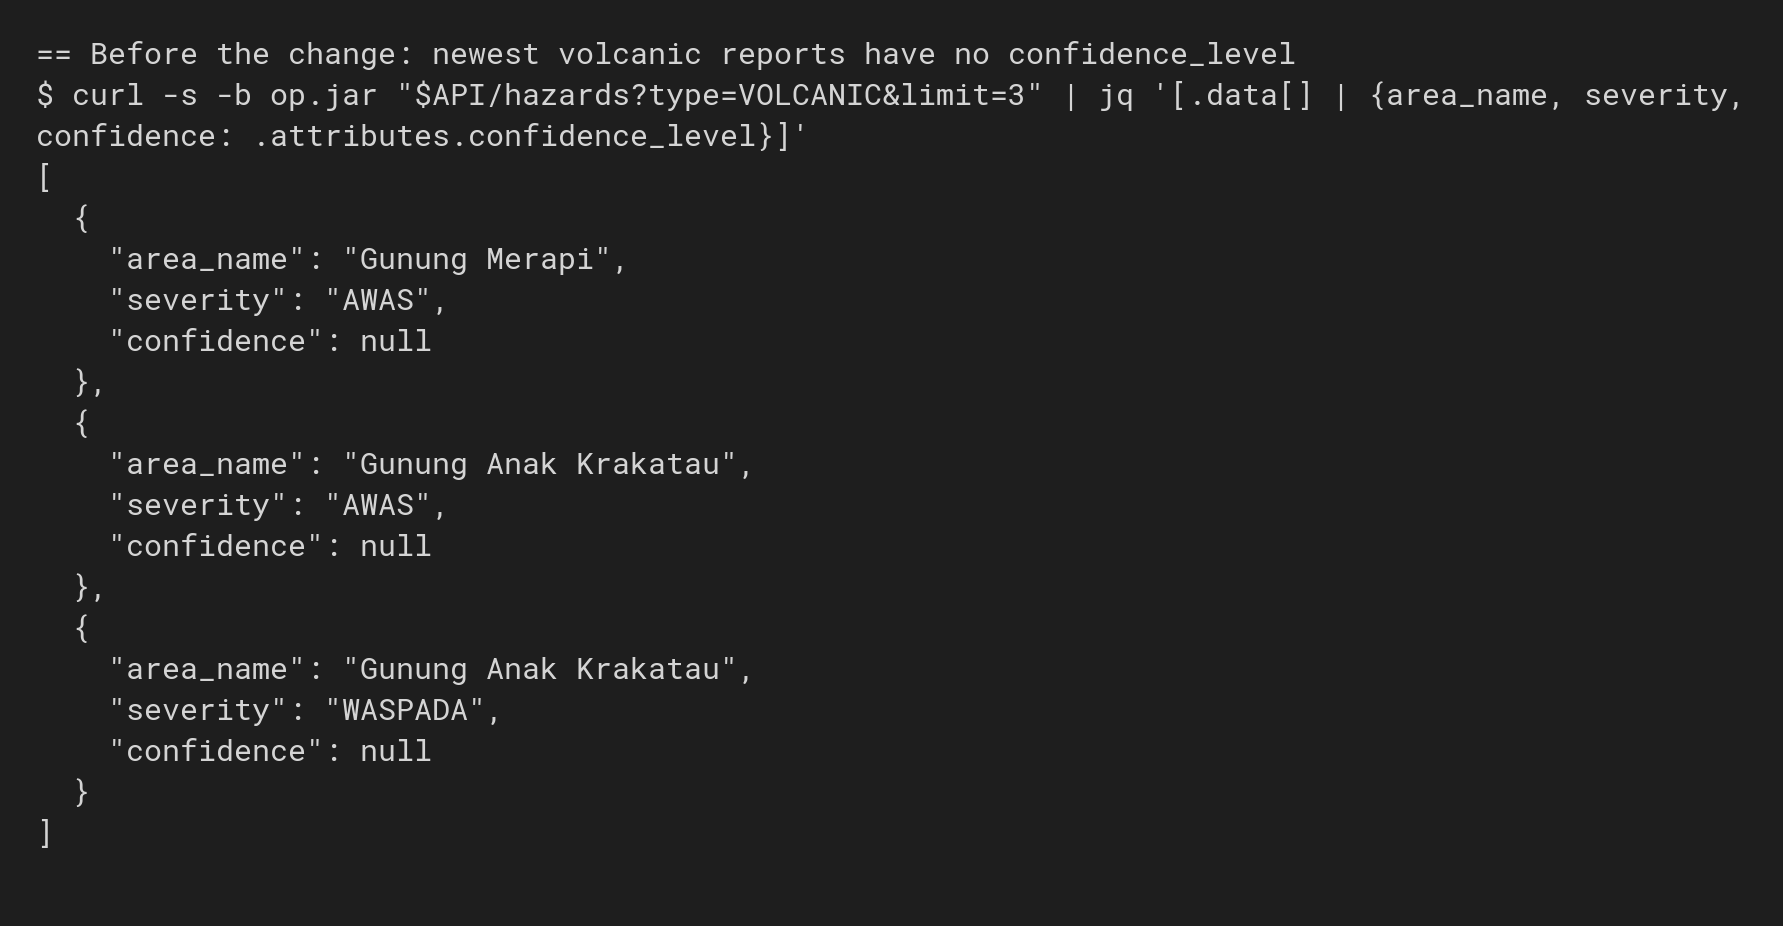
\includegraphics[width=\linewidth,height=0.72\textheight,keepaspectratio]{figures/bukti/vi1.png}
\caption{Tiga laporan vulkanik terbaru sebelum perubahan skema}
\end{figure}

\subsection{Picu Perubahan Skema PVMBG}

Perubahan skema dipicu lewat endpoint admin PVMBG tanpa me-restart mock maupun Aggregator.

\begin{figure}[H]
\centering
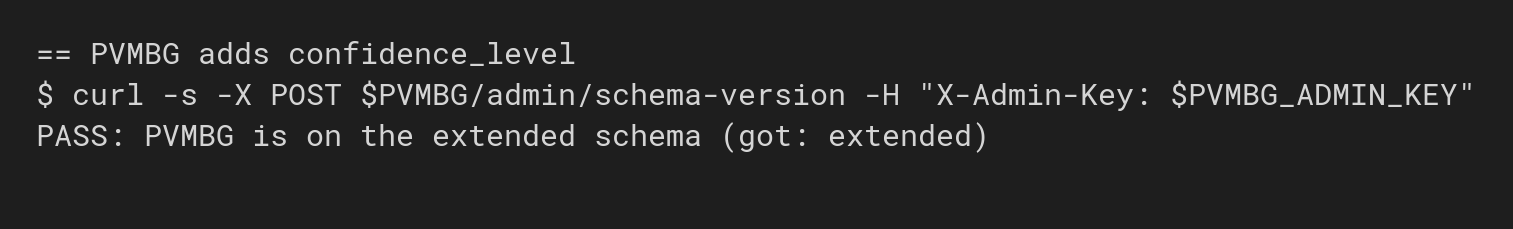
\includegraphics[width=\linewidth,height=0.72\textheight,keepaspectratio]{figures/bukti/vi2.png}
\caption{Memicu perubahan skema PVMBG}
\end{figure}

\subsection{Aggregator Tetap Menghasilkan HazardEvent}

Setelah perubahan, laporan baru membawa \texttt{confidence\_level} di \texttt{attributes}, laporan lama tetap terbaca, dan waktu mulai kontainer Aggregator tidak berubah. Tabel \texttt{hazard\_events} menyimpan rekaman sebelum dan sesudah perubahan berdampingan tanpa migrasi (kolom \texttt{has\_confidence} adalah hasil pemeriksaan \texttt{attributes ? 'confidence\_level'}).

\begin{figure}[H]
\centering
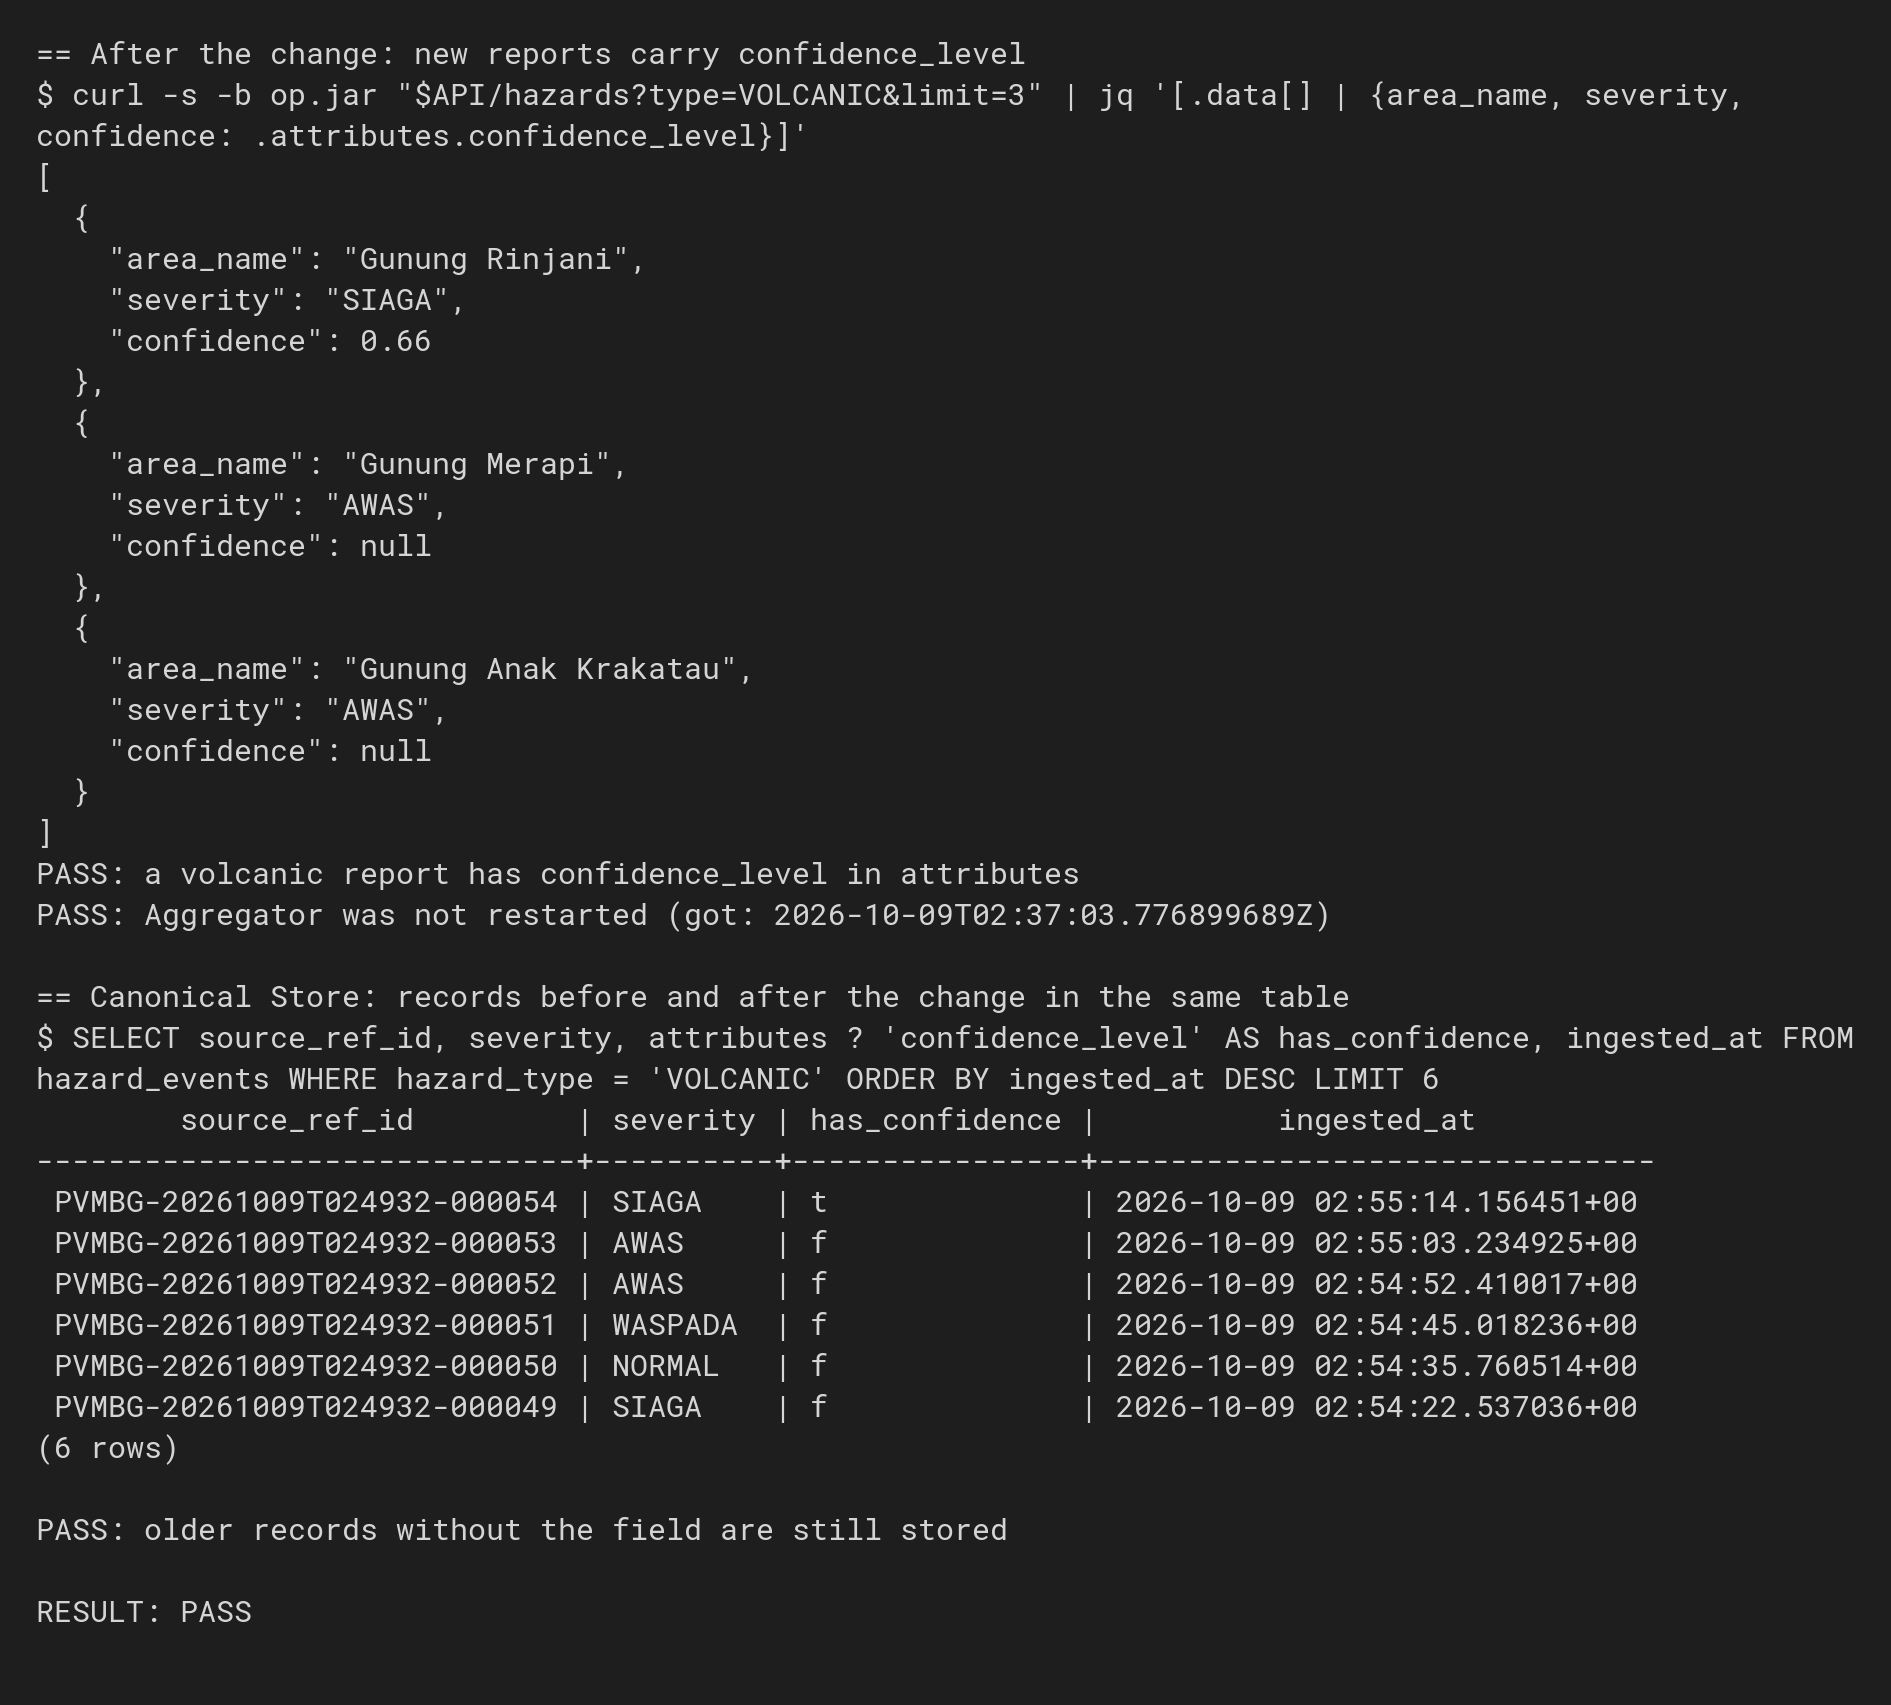
\includegraphics[width=\linewidth,height=0.72\textheight,keepaspectratio]{figures/bukti/vi3.png}
\caption{Laporan sesudah perubahan dan isi tabel \texttt{hazard\_events}}
\end{figure}


\chapter{Problem 2 - Concurrency, Availability, \& Graceful Degradation}

\section{Rancangan Solusi}

\subsection{Pemisahan Jalur Ingest dan Jalur Pelayanan}

Sistem memisahkan dua jalur yang sebelumnya menyatu dalam satu alur:

\begin{itemize}
\tightlist
\item
  Jalur ingest: Aggregator melakukan polling ke BMKG dan PVMBG di belakang, memetakan hasilnya ke HazardEvent, lalu menyimpannya ke Canonical Store.\\
\item
  Jalur pelayanan: permintaan client diterima Client-Facing API, diteruskan ke read API milik Aggregator, dan dijawab dari Canonical Store.
\end{itemize}

Dengan pemisahan ini, permintaan client tidak pernah menunggu respons BMKG maupun PVMBG secara langsung. Latensi PVMBG (500 ms-3 detik) hanya berdampak pada seberapa cepat data vulkanik baru masuk ke store, bukan pada latensi permintaan client.

Endpoint penyajian dipisah berdasarkan jenis bahaya:

\begin{itemize}
\tightlist
\item
  GET /hazards?type=SEISMIC -\textgreater{} hanya membaca data bersumber BMKG\\
\item
  GET /hazards?type=VOLCANIC -\textgreater{} hanya membaca data bersumber PVMBG
\end{itemize}

Permintaan ``BMKG-only'' pada kriteria penyelesaian merujuk ke endpoint seismik, yang sama sekali tidak menyentuh status maupun data PVMBG.

\subsection{Poller Independen per Sumber}

Setiap sumber memiliki poller sendiri yang berjalan sebagai \textit{goroutine} terpisah di dalam Aggregator:

\begin{itemize}
\tightlist
\item
  Poller BMKG dan poller PVMBG memiliki loop, interval, dan timeout masing-masing, sehingga poller BMKG tidak pernah menunggu poller PVMBG.\\
\item
  Setiap poller hanya menjalankan satu panggilan dalam satu waktu (single in-flight), panggilan berikutnya baru dimulai setelah panggilan sebelumnya selesai atau terkena timeout. Waktu tunggu sebelum panggilan berikutnya dihitung sebagai interval polling dikurangi durasi panggilan sebelumnya. Jika durasi panggilan melebihi interval, panggilan berikutnya langsung dijalankan tanpa menunggu. Dengan demikian, jarak antar panggilan tetap sebesar interval saat sumber normal, tidak melebihi durasi timeout saat sumber melambat, dan panggilan tidak pernah menumpuk.\\
\item
  Setiap panggilan keluar diberi timeout eksplisit. Panggilan yang melewati timeout dibatalkan dan dihitung sebagai kegagalan.\\
\item
  Setiap poller dibungkus circuit breaker tersendiri.
\end{itemize}

Model konkurensi yang digunakan adalah \textit{goroutine} Go di atas I/O jaringan yang tidak memblokir \textit{thread} sistem operasi: \textit{goroutine} yang menunggu respons hanya diparkir oleh \textit{runtime}, sehingga poller dan penanganan permintaan client dapat berjalan bersamaan tanpa saling menahan.

\subsection{Pembatasan Konkurensi}

Untuk mencegah lonjakan akses menghabiskan resource, sistem menerapkan batas di beberapa lapisan:

\begin{itemize}
\tightlist
\item
  Global concurrency cap (Client-Facing API dan read API Aggregator): jumlah permintaan yang diproses bersamaan dibatasi oleh semaphore. Permintaan yang datang saat kapasitas penuh langsung ditolak dengan HTTP 429 beserta header Retry-After (load shedding).\\
\item
  Rate limit per client (Client-Facing API): setiap identitas client (Media, Tim Lapangan, BNPB Ops) dibatasi dengan algoritma token bucket. Lapisan ini berfungsi sebagai pembagi kapasitas yang adil agar satu client tidak memonopoli sistem, bukan sebagai pelindung kapasitas utama.\\
\item
  Timeout per hop: setiap panggilan Client-Facing API -\textgreater{} Aggregator dan Aggregator -\textgreater{} Canonical Store memiliki batas waktu, sehingga tidak ada permintaan yang menggantung dan menahan resource.\\
\item
  Connection pool terbatas: koneksi HTTP ke Aggregator dan koneksi ke Canonical Store memakai pool berukuran tetap.
\end{itemize}

\subsection{Status Kebaruan Data dan Degradasi}

Aggregator menyimpan status untuk setiap sumber.

\begin{longtable}[]{|>{\raggedright\arraybackslash}p{\dimexpr(\linewidth-4\tabcolsep)/2\relax}|>{\raggedright\arraybackslash}p{\dimexpr(\linewidth-4\tabcolsep)/2\relax}|}
\hline
Attributes & Value \\
\hline
\endhead
\endlastfoot
source & BMKG \\
\hline
status & UP, DEGRADED, atau DOWN \\
\hline
last\_success\_at & Waktu polling terakhir yang berhasil \\
\hline
stale\_since & Waktu data mulai dianggap basi (null bila UP) \\
\hline
consecutive\_fail & jumlah kegagalan polling berturut-turut \\
\hline
\end{longtable}

Status ini dikendalikan oleh circuit breaker per sumber:

\begin{itemize}
\tightlist
\item
  CLOSED: polling berjalan normal. Status UP, atau DEGRADED bila ada kegagalan berturut-turut yang masih di bawah ambang.\\
\item
  OPEN: setelah N kegagalan berturut-turut, breaker terbuka dan status menjadi DOWN. Polling ke sumber dihentikan sementara (fail fast) agar resource tidak terbuang untuk sumber yang mati, dan stale\_since diisi dengan last\_success\_at.\\
\item
  HALF-OPEN: setelah durasi tertentu, satu panggilan percobaan dikirim. Jika berhasil, breaker kembali CLOSED, status kembali UP, dan stale\_since dikosongkan tanpa restart. Jika gagal, breaker kembali OPEN.
\end{itemize}

Perilaku respons berdasarkan kondisi sumber:

\begin{longtable}[]{|>{\raggedright\arraybackslash}p{\dimexpr(\linewidth-4\tabcolsep)/2\relax}|>{\raggedright\arraybackslash}p{\dimexpr(\linewidth-4\tabcolsep)/2\relax}|}
\hline
Kondisi & Respons \\
\hline
\endhead
\endlastfoot
Sumber UP & 200, data terbaru \\
\hline
Sumber DOWN, store berisi data & 200, data terakhir + meta.stale\_since \\
\hline
Sumber DOWN, store kosong & 503, body eksplisit: sumber tidak tersedia \\
\hline
Permintaan untuk sumber lain & tidak terpengaruh \\
\hline
\end{longtable}

Setiap respons menyertakan metadata kebaruan, contoh:

\begin{codebox}
{
"data": [ ...HazardEvent... ],
"meta": {
     "source": "PVMBG",
     "source_status": "DOWN",
     "last_success_at": "2026-10-01T10:15:02Z",
     "stale_since": "2026-10-01T10:15:02Z" }
}
\end{codebox}

Dengan demikian, selama outage PVMBG permintaan seismik tetap dilayani normal, permintaan vulkanik dijawab dengan data terakhir beserta penanda kebaruan, tidak ada respons 500, dan tidak ada permintaan yang menggantung hingga timeout client.

\subsection{Parameter Konfigurasi}

Seluruh parameter dibaca dari environment variable:

\begin{longtable}[]{|>{\raggedright\arraybackslash}p{\dimexpr(\linewidth-6\tabcolsep)/3\relax}|>{\raggedright\arraybackslash}p{\dimexpr(\linewidth-6\tabcolsep)/3\relax}|>{\raggedright\arraybackslash}p{\dimexpr(\linewidth-6\tabcolsep)/3\relax}|}
\hline
Variabel & Default & Keterangan \\
\hline
\endhead
\endlastfoot
POLL\_INTERVAL\_MS & 3000 & Interval polling per sumber \\
\hline
POLL\_TIMEOUT\_MS & 4000 & Timeout satu panggilan polling \\
\hline
CB\_FAILURE\_THRESHOLD & 3 & Kegagalan berturut-turut sebelum OPEN \\
\hline
CB\_OPEN\_DURATION\_MS & 10000 & Durasi OPEN sebelum HALF-OPEN \\
\hline
AGGREGATOR\_MAX\_INFLIGHT\_REQUESTS & 100 & Global concurrency cap (semaphore) pada read API Aggregator \\
\hline
CLIENT\_FACING\_API\_MAX\_INFLIGHT\_REQUESTS & 100 & Global concurrency cap (semaphore) pada Client-Facing API \\
\hline
RATE\_LIMIT\_RPS & 50 & Token bucket per akun \\
\hline
AUTH\_RATE\_LIMIT\_RPS & 10 & Token bucket per alamat IP untuk login dan registrasi \\
\hline
UPSTREAM\_TIMEOUT\_MS & 1000 & Timeout Client-Facing API -\textgreater{} Aggregator \\
\hline
DB\_POOL\_SIZE & 20 & Ukuran connection pool Canonical Store \\
\hline
\end{longtable}

\section{Alasan Keputusan}

\subsection{Pemisahan Jalur Ingest dan Jalur Akses}

Alternatif yang dipertimbangkan:

\begin{itemize}
\tightlist
\item
  Proxy langsung: setiap permintaan client diteruskan secara real-time ke BMKG/PVMBG. Ini adalah pendekatan prototipe awal dan merupakan sumber utama head-of-line blocking, karena latensi client ikut menanggung latensi sumber yang paling lambat.\\
\item
  Scatter-gather parallel per permintaan: BMKG dan PVMBG dipanggil paralel saat ada permintaan. Pendekatan ini menghilangkan urutan sekuensial, tetapi permintaan yang membutuhkan PVMBG tetap menunggu hingga 3 detik, setiap permintaan client melipatgandakan beban ke sumber, dan outage sumber langsung terasa oleh client.\\
\item
  Cache dengan TTL di depan sumber: mengurangi beban, tetapi saat cache kedaluwarsa permintaan kembali menunggu sumber (cache miss), sehingga latensi menjadi tidak konsisten.
\end{itemize}

Pendekatan yang dipilih (polling di \emph{background}, client membaca dari \emph{Canonical Store}) dipilih karena latensi client sepenuhnya lepas dari latensi dan ketersediaan sumber. Selain itu, spesifikasi sudah menetapkan pola ingest berupa polling, sehingga \emph{Canonical Store} secara alami menjadi sumber jawaban bagi client.

Trade-off:\\
data yang diterima client bersifat eventually consistent, dengan keterlambatan maksimal sebesar interval polling ditambah latensi sumber. Untuk kebutuhan koordinasi kebencanaan dengan interval 2-5 detik, keterlambatan ini dapat diterima.

\subsection{Model Konkurensi Goroutine dengan I/O Non-Blocking}

Alternatif yang dipertimbangkan:

\begin{itemize}
\tightlist
\item
  Thread-per-request: sederhana, tetapi setiap permintaan yang menunggu I/O menahan satu thread sistem operasi beserta memorinya. Pada lonjakan akses, jumlah thread tumbuh tanpa batas dan menjadi penyebab \emph{resource exhaustion} itu sendiri.\\
\item
  \emph{Worker pool} dengan thread tetap: jumlah thread terkendali, tetapi thread tetap menganggur selama menunggu I/O, sehingga kapasitas efektif terbatas pada jumlah thread.\\
\item
  \emph{Event loop} tunggal: biaya per koneksi kecil, tetapi satu operasi \emph{blocking} atau komputasi berat menahan seluruh \emph{loop}.
\end{itemize}

Beban kerja sistem didominasi I/O (panggilan jaringan ke sumber, Aggregator, dan Canonical Store), bukan komputasi. Go menjalankan setiap poller dan setiap permintaan sebagai \emph{goroutine} yang dijadwalkan \emph{runtime} di atas sedikit thread. Ketika sebuah \emph{goroutine} menunggu jaringan, \emph{runtime} memarkirnya dan memakai thread itu untuk \emph{goroutine} lain. Hasilnya sama dengan I/O non-blocking, dengan kode yang ditulis berurutan dan tanpa \emph{callback}.

Trade-off: jumlah \emph{goroutine} tidak dibatasi oleh bahasa, sehingga pembatasan harus datang dari sistem. Itulah alasan semaphore, \emph{rate limit}, dan \emph{timeout} per hop dipasang di depan setiap jalur permintaan. \emph{Goroutine} juga bukan jaminan paralelisme untuk komputasi berat, tetapi pemetaan skema bersifat ringan sehingga risikonya dinilai kecil.

\subsection{Poller Independen dengan Single In-Flight}

Alternatif yang dipertimbangkan:

\begin{itemize}
\tightlist
\item
  Satu loop polling sekuensial (BMKG lalu PVMBG): siklus BMKG tertahan oleh PVMBG, sehingga data seismik ikut terlambat masuk ke store.\\
\item
  Satu loop yang memanggil kedua sumber secara paralel lalu menunggu keduanya: urutan tidak lagi sekuensial, tetapi siklus berikutnya tetap menunggu sumber yang paling lambat.
\end{itemize}

Poller terpisah per sumber membuat laju ingest BMKG sama sekali tidak bergantung pada PVMBG. Aturan single in-flight dipilih agar panggilan ke sumber yang melambat tidak menumpuk dan tidak memperparah beban pada sumber tersebut.

Trade-off: saat sumber melambat, sebagian siklus polling dilewati sehingga data baru dari sumber tersebut masuk sedikit lebih lambat.

\subsection{Load Shedding pada Global Concurrency Cap}

Alternatif yang dipertimbangkan:

\begin{itemize}
\tightlist
\item
  Tanpa batas: setiap permintaan diterima dan diproses. Ini adalah kondisi yang menyebabkan resource exhaustion.\\
\item
  Antrian tanpa batas: permintaan tidak ditolak, tetapi antrian tumbuh terus saat lonjakan, latensi meningkat tanpa batas, dan memori habis.\\
\item
  Antrian berbatas dengan waktu tunggu: permintaan menunggu giliran, tetapi menambah latensi pada semua permintaan saat sistem sibuk.
\end{itemize}

Penolakan langsung dengan HTTP 429 dipilih karena menjaga latensi permintaan yang diterima tetap rendah dan memberi sinyal yang jelas kepada client untuk mencoba kembali (Retry-After). Sistem tetap melayani sebagian permintaan dengan baik.

Trade-off: sebagian client menerima 429 saat puncak beban dan perlu melakukan retry.

\subsection{Rate Limiting Token Bucket per Client}

Alternatif yang dipertimbangkan:

\begin{itemize}
\tightlist
\item
  Fixed window: sederhana, tetapi memungkinkan lonjakan dua kali lipat di sekitar batas window.\\
\item
  Sliding window log: akurat, tetapi harus menyimpan timestamp setiap permintaan sehingga boros memori.\\
\item
  Leaky bucket: menghasilkan laju keluaran yang rata, tetapi permintaan diantrikan terlebih dahulu sehingga menambah latensi dan berisiko melanggar target p95 \textless{} 300 ms.\\
\item
  Sliding window counter: menyeimbangkan akurasi dan memory dengan weighted average antar window, tetapi hasilnya tetap estimasi (asumsi distribusi request merata di window sebelumnya) sehingga bisa sedikit meleset saat traffic bursty/tidak uniform.
\end{itemize}

Token bucket dipilih karena mengizinkan burst singkat yang wajar, tidak menambah latensi pada permintaan yang lolos, dan hanya membutuhkan dua nilai per client (jumlah token dan waktu isi ulang terakhir).

Kunci rate limit berupa client\_id dari klaim JWT, bukan alamat IP, karena beberapa client dapat berbagi IP yang sama (misalnya di balik NAT atau saat load testing) dan identitas client sudah terverifikasi oleh Client-Facing API.

Trade-off: state token bucket disimpan in-memory sehingga hilang saat Client-Facing API di-restart dan tidak dapat dibagi antar-instance. Karena Client-Facing API berjalan sebagai satu instance pada M1, hal ini dapat diterima (lihat 7.3).

\subsection{Circuit Breaker dan Respons Stale dengan Penanda}

Alternatif yang dipertimbangkan:

\begin{itemize}
\tightlist
\item
  Mengembalikan error saat sumber mati: sederhana, tetapi membuang data terakhir yang masih berguna. Ini adalah perilaku yang menyebabkan dashboard BNPB kosong.\\
\item
  Menyajikan data terakhir tanpa penanda: client tidak dapat membedakan data terkini dari data basi, yang berbahaya dalam konteks kebencanaan karena status gunung api dapat berubah selama outage.\\
\item
  Retry terus-menerus tanpa circuit breaker: membuang resource untuk sumber yang sudah jelas mati dan memperbanyak error log.
\end{itemize}

Kombinasi circuit breaker dan respons stale dengan penanda (stale\_since, source\_status) dipilih karena data terakhir tetap tersedia bagi client, client mengetahui secara eksplisit sejak kapan data tersebut tidak diperbarui, dan sistem berhenti membuang resource untuk sumber yang mati. Status HALF-OPEN memungkinkan pemulihan otomatis tanpa restart ketika sumber kembali hidup.\\
Respons 503 dengan body eksplisit dipilih untuk kondisi store kosong, karena mengembalikan 200 dengan data kosong dapat disalahartikan sebagai ``tidak ada aktivitas vulkanik''.

Trade-off: deteksi outage tidak instan, melainkan membutuhkan N kegagalan berturut-turut (CB\_FAILURE\_THRESHOLD). Pemulihan juga tertunda hingga durasi OPEN berakhir (CB\_OPEN\_DURATION\_MS). Nilai keduanya dapat dikonfigurasi untuk menyeimbangkan kecepatan deteksi dan ketahanan terhadap gangguan sesaat.

\section{Batasan Yang Disadari}

\subsection{Data Bersifat Eventual Consistent}

Client membaca dari Canonical Store, sehingga data yang diterima tertinggal paling lama sebesar interval polling ditambah latensi sumber. Hal ini merupakan konsekuensi dari pola ingest polling yang ditetapkan spesifikasi, dan dengan interval 2-5 detik keterlambatan ini masih dapat diterima untuk kebutuhan koordinasi.

\subsection{Deteksi Outage Tidak Instan}

Circuit breaker baru terbuka setelah CB\_FAILURE\_THRESHOLD kegagalan berturut-turut, sehingga selama jeda tersebut data vulkanik masih disajikan dengan status UP. Ambang ini sengaja dipasang agar gangguan sesaat tidak langsung dianggap outage. Setelah status berubah, stale\_since tetap akurat karena diisi dengan last\_success\_at.

\subsection{Sumber yang Sangat Lambat Diperlakukan Sama dengan Sumber yang Mati}

Panggilan yang melewati POLL\_TIMEOUT\_MS dihitung sebagai kegagalan, karena sumber yang lambat maupun mati sama-sama tidak menghasilkan data tepat waktu. Nilai default timeout sengaja diatur di atas delay maksimum PVMBG pada spesifikasi (3 detik).

\subsection{Load shedding tidak memprioritaskan client}

Global concurrency cap berlaku sama untuk semua client, sehingga saat beban puncak permintaan Tim Lapangan dapat ditolak sama seperti permintaan Media.

\subsection{Satu instance per service dan state in-memory}

Client-Facing API dan Aggregator masing-masing berjalan sebagai satu instance, dengan state token bucket dan status sumber disimpan in-memory. State ini hilang saat restart dan akan terbentuk ulang dari permintaan dan hasil polling berikutnya. Skala horizontal membutuhkan penyimpanan state bersama (misalnya Redis) yang menambah komponen baru, sedangkan satu instance sudah cukup untuk kriteria M1.

\subsection{Aggregator dan Canonical Store Merupakan Dependensi Jalur Akses}

Jika Aggregator atau Canonical Store mati, seluruh permintaan data tidak dapat dilayani. Client-Facing API mengembalikan 503 eksplisit tanpa menggantung, tetapi tidak menyediakan data cadangan.

\subsection{Cap konkurensi bersifat global, bukan per client}

Satu client yang mengirim \textit{body} sangat lambat ke \texttt{POST /auth/login} memegang satu slot sampai batas baca 10 detik. \textit{Throttle} per IP (10 permintaan per detik) cukup longgar untuk menjaga sekitar 100 slot tetap terisi, dan selama itu permintaan lain selain \texttt{/health} menerima 429. Efeknya berakhir beberapa detik setelah client berhenti. Skenario ini belum diuji.

\subsection{Kebaruan data dilaporkan per sumber}

Kesegaran data dibatasi interval polling. Status basi dilaporkan per sumber lewat \texttt{stale\_since}, bukan per rekaman.

\subsection{Hasil load testing bergantung pada lingkungan pengujian}

Load testing dijalankan pada satu mesin yang juga menjalankan seluruh container, sehingga load generator dan sistem berbagi CPU dan memori. Angka yang dilaporkan bertujuan membuktikan perilaku sistem di bawah beban, bukan mengukur kapasitas produksi.

\section{Bukti Penyelesaian}

\subsection{Uji p95 BMKG-only saat PVMBG delay 3 detik}

\textless placeholder\textgreater{}

\subsection{Load Testing (≥50 koneksi, 60 detik)}

\textless placeholder\textgreater{}

\subsection{Demo Outage PVMBG}

\textless placeholder\textgreater{}

\section{Model Konkurensi dan Mitigasi Kegagalan}

\subsection{Model Konkurensi}

Sistem menggunakan \emph{goroutine} Go di atas I/O jaringan yang tidak memblokir thread. Beban kerja sistem didominasi operasi I/O (panggilan jaringan ke sumber, Aggregator, dan Canonical Store), bukan komputasi, sehingga paralelisme tidak menjadi fokus rancangan. Poller BMKG, poller PVMBG, dan penanganan permintaan client berjalan sebagai \emph{goroutine} independen, dengan jumlah permintaan bersamaan dibatasi oleh semaphore.

\subsection{Mitigasi Head-of-Line Blocking}

Client tidak pernah memicu panggilan langsung ke BMKG maupun PVMBG. Permintaan client dijawab Aggregator dari Canonical Store, sehingga latensi PVMBG tidak masuk ke jalur permintaan client. Poller per sumber juga berjalan independen, sehingga ingest data seismik tidak tertahan oleh PVMBG yang lambat (7.1.1, 7.1.2).

\subsection{Mitigasi Resource Exhaustion}

Semaphore membatasi jumlah permintaan yang diproses bersamaan, dan permintaan yang melebihi kapasitas langsung ditolak dengan HTTP 429. Rate limiting per client dengan token bucket mencegah satu client memonopoli kapasitas, sementara timeout di setiap hop dan connection pool terbatas mencegah permintaan menggantung dan menahan resource (7.1.3).

\subsection{Mitigasi Ketiadaan Degradasi Terkendali}

Circuit breaker per sumber mendeteksi sumber yang mati secara otomatis di level polling, lalu mencatat stale\_since. Selama sumber DOWN, data sumber tersebut dijawab dari Canonical Store beserta stale\_since, sedangkan sumber lain tidak terpengaruh. Setelah sumber hidup kembali, circuit breaker memulihkan status secara otomatis tanpa restart (7.1.4).

\section{Konfigurasi dan Tooling Load Testing}

Uji beban memakai k6 yang dijalankan dari \textit{image} Docker (\texttt{grafana/k6}), sehingga tidak perlu dipasang. Skrip \texttt{tests/load/run.sh} menyalakan seluruh sistem dalam proyek Compose terpisah (\texttt{hazard-load}) dengan \texttt{.env.example}, mengatur PVMBG menjawab setelah tepat 3 detik, menaikkan TTL \textit{access token} agar sesi tidak kedaluwarsa selama uji, menjalankan skenario di \texttt{tests/load/p2.js}, lalu menghapus sistem. Ringkasan disimpan di \texttt{tests/load/results/}.

\begin{longtable}[]{|>{\raggedright\arraybackslash}p{0.2\linewidth}|>{\raggedright\arraybackslash}p{0.42\linewidth}|>{\raggedright\arraybackslash}p{0.28\linewidth}|}
\hline
Skenario & Pola beban & Ambang \\
\hline
\endhead
\texttt{bmkg\_only} & 20 permintaan per detik selama 30 detik ke \texttt{GET /hazards?type=SEISMIC} saat PVMBG menjawab setelah 3 detik & p95 di bawah 300 ms, galat di bawah 1\% \\
\hline
\texttt{mixed} & 50 koneksi paralel selama 60 detik, dimulai pada detik ke-35, campuran seismik, vulkanik, dengan dan tanpa \texttt{fields}, dan \texttt{/health}, dengan jeda sekitar 1 detik per koneksi & Galat di luar 429 di bawah 1\% \\
\hline
\end{longtable}

Galat dihitung sebagai respons selain 200 dan 429. Jumlah tiap kode status (200, 401, 429, 500, 502, 503, 504) dilaporkan pada ringkasan agar penolakan terkontrol tetap terlihat. Kedua skenario memakai satu akun Operator, sehingga 50 koneksi dengan jeda sekitar 1 detik meminta sekitar 50 permintaan per detik, mendekati batas \texttt{RATE\_LIMIT\_RPS}. Angka throughput, p50, p95, dan p99 dilaporkan pada Bukti Penyelesaian.

\chapter{Problem 3 - Service-to-Service Authentication \& Trust}

\section{Rancangan Solusi}

\subsection{Otentikasi dan Otorisasi antar Servis}

\textbf{Flow PVMBG:}

\begin{enumerate}
\def\labelenumi{\arabic{enumi}.}
\tightlist
\item
  PVMBG menyediakan layanan untuk mengakses \emph{resource protected} mereka. Perlu daftar akun terlebih dahulu.\\
\item
  Setelah daftar akun dan mengisi beberapa data berkaitan dengan instansi/perusahaan untuk memverifikasi penggunaan, admin PVMBG akan memverifikasi pendaftaran.\\
\item
  Apabila sudah terverifikasi, BNPB akan mendapat client ID dan client secret.\\
\item
  Setelah client ID dan client secret didapatkan, BNPB \emph{generate} one time code (misalnya melalui web interface PVMBG) agar bisa mendapat access token untuk pertama kalinya:
\end{enumerate}

\begin{longtable}[]{|>{\raggedright\arraybackslash}p{\dimexpr(\linewidth-4\tabcolsep)/2\relax}|>{\raggedright\arraybackslash}p{\dimexpr(\linewidth-4\tabcolsep)/2\relax}|}
\hline
\texttt{URL} & \texttt{/oauth/token} \\
\hline
\endhead
\endlastfoot
\texttt{Method} & \texttt{HTTP\ POST} \\
\hline
\textbf{\texttt{Header}} & \\
\hline
\texttt{Authorization} & \texttt{Basic\ Y2xpZW50X2lkOmNsaWVudF9zZWNyZXQ=} \\
\hline
\textbf{\texttt{Request\ Body}} & \\
\hline
\texttt{code} & \texttt{\textless{}one\_time\_code\textgreater{}} \\
\hline
\texttt{grant\_type} & \texttt{authorization\_code} \\
\hline
\end{longtable}

Dengan authorization header bernilai \textless client\_id\textgreater:\textless client\_secret\textgreater{} dalam format base64

Akan dikembalikan:

\begin{codebox}
{
    "access_token" : "<access_token>",
    "refresh_token" : "<refresh_token>",
    "expires_in" : 60
}
\end{codebox}

Dengan ketentuan bahwa access token yang dipakai oleh service BNPB untuk mengakses resource (dalam Authorization: Bearer). Selanjutnya, refresh token dipakai untuk mendapatkan access token baru (asumsinya satu client hanya mempunyai satu access token yang valid dalam waktu yang sama):

\begin{longtable}[]{|>{\raggedright\arraybackslash}p{\dimexpr(\linewidth-4\tabcolsep)/2\relax}|>{\raggedright\arraybackslash}p{\dimexpr(\linewidth-4\tabcolsep)/2\relax}|}
\hline
\texttt{URL} & \texttt{/oauth/token} \\
\hline
\endhead
\endlastfoot
\texttt{Method} & \texttt{HTTP\ POST} \\
\hline
\textbf{\texttt{Header}} & \\
\hline
\texttt{Authorization} & \texttt{Basic\ Y2xpZW50X2lkOmNsaWVudF9zZWNyZXQ=} \\
\hline
\textbf{\texttt{Request\ Body}} & \\
\hline
\texttt{grant\_type} & \texttt{refresh\_token} \\
\hline
\texttt{refresh\_token} & \texttt{\textless{}refresh\_token\textgreater{}} \\
\hline
\end{longtable}

Akan dikembalikan:

\begin{codebox}
{
    "access_token" : "<new_access_token>",
    "refresh_token" : "<new_refresh_token>",
    "expires_in" : 60
}
\end{codebox}

Catatan: \texttt{expires\_in} bernilai 60 detik untuk keperluan demonstrasi. Mock PVMBG hanya mengizinkan satu pasangan token yang valid untuk satu client, sehingga setelah refresh, token lama langsung ditolak.

Agar token dan refresh token persists through multiple deployment, volume perlu dikonfigurasi dalam file docker compose.

\textbf{Flow BMKG:}

\begin{enumerate}
\def\labelenumi{\arabic{enumi}.}
\tightlist
\item
  BMKG menyediakan servis developer API. BNPB perlu daftar akun developer terlebih dahulu dan verifikasi perusahaan/instansi.\\
\item
  Apabila sudah terverifikasi, BNPB dapat create new API key yang diberi nama (mis. bnpb-app-key). API key hanya muncul sekali di interface, sehingga BNPB perlu copy key tersebut dan simpan dalam .env mereka.\\
\item
  API key dapat dipakai dengan menyertakan header X-BMKG-Key dalam GET HTTP request ke BMKG. Tanpa X-BMKG-Key, permintaan akan ditolak.\\
\item
  API Key dapat direvoke kapanpun oleh akun BNPB.
\end{enumerate}

\subsection{Otentikasi dan Otorisasi Client ke Service}

BNPB mempunyai IdP sendiri untuk otorisasi dan otentikasi client downstream yang menggunakan HMAC Signed JWT sebagai token otorisasinya. Pengguna dapat mendaftarkan akun sebagai media. Akun operator di-\emph{seed} ke dalam database, sedangkan akun lapangan ditambahkan oleh operator. Diasumsikan tidak perlu verifikasi email untuk pendaftaran akun. Setelah akun berhasil didaftar, pengguna dapat login menggunakan email dan password masing-masing. Flow requestnya:

\begin{enumerate}
\def\labelenumi{\arabic{enumi}.}
\tightlist
\item
  Pengguna request login\\
\item
  Request masuk ke API Gateway\\
\item
  Request login diarahkan ke IdP\\
\item
  IdP verifikasi email dan hash(password + secret\_salt)\\
\item
  Jika password benar, IdP mengembalikan set-cookie HttpOnly sebuah JWT berupa
\end{enumerate}

\begin{codebox}
Header:
{ "alg": "HS256", "typ": "JWT" }

Payload:
{
  "name": "Jane Doe",
  "email": "jane@example.com",
  "role": "Media/Lapangan/Operator",
  "iat": 1727360297,
  "exp": 1727360357
}

Base64HeaderAndPayload = Base64(Header) + “.” + Base64(Payload)

Signature: HMACSHA256(Base64HeaderAndPayload)

Yang dikembalikan:
Base64HeaderAndPayload + “.” + Signature
\end{codebox}

Nilai exp (expired at, unix timestamp) adalah iat ditambah ACCESS\_TOKEN\_TTL\_S, default 60 detik, dan berlaku sama untuk semua role.

\begin{enumerate}
\def\labelenumi{\arabic{enumi}.}
\setcounter{enumi}{5}
\tightlist
\item
  Setelah login, setiap client request menggunakan cookie tersebut. Setiap request masuk API Gateway, JWT langsung diverifikasi oleh API Gateway.\\
\item
  Jika JWT valid, request langsung diteruskan ke service BNPB
\end{enumerate}

Selain itu terdapat mekanisme refresh token. JWT dapat direfresh menggunakan refresh token. Refresh token bersifat stateful yang disimpan dalam user DB dalam IdP. Jadi skema database akan seperti:

\begin{codebox}
CREATE TABLE refresh_tokens (
       refresh_token        VARCHAR(64) PRIMARY KEY,
       user_id              VARCHAR(255) NOT NULL,
       
       FOREIGN KEY (user_id) REFERENCES users(user_id)
)
\end{codebox}

Panjang Varchar(64) merupakan contoh saja. Saat login, refresh token juga di set-cookie bersama JWT. Refresh token yang dikembalikan juga disimpan dalam DB seperti skema di atas. Selama pengguna tidak logout, refresh token yang disimpan dalam DB akan terus ada. Refresh token dalam DB hanya dihapus dalam:

\begin{enumerate}
\def\labelenumi{\arabic{enumi}.}
\tightlist
\item
  Request refresh JWT (technically diupdate sih), dan\\
\item
  Logout akun
\end{enumerate}

Request refresh JWT itu harus otomatis terjadi setiap kali pengguna mengirim sebuah request tetapi JWT itu expired. Flownya adalah seperti berikut ini:

\begin{enumerate}
\def\labelenumi{\arabic{enumi}.}
\tightlist
\item
  Pengguna mengirim request dengan JWT yang expired bersama refresh token yang valid.\\
\item
  Client Facing API mendeteksi bahwa JWT tidak valid. Request disimpan dalam memory, kemudian memanggil RPC Refresh pada IdP dengan hanya meneruskan refresh token.\\
\item
  IdP fetch where refresh\_token = refresh\_token dalam DB sambil join tabel user. Apabila ada, artinya refresh token masih valid. Kemudian refresh token bersama JWT-nya dirotasi. Refresh token lama diupdate menjadi refresh token baru, kemudian JWT dan refresh token baru dikembalikan ke Client Facing API.\\
\item
  Gateway menerima JWT dan refresh token baru, kemudian inject JWT yang valid ke GET Request. Request tersebut diteruskan ke servis berikutnya.\\
\item
  Setelah menerima response, Client Facing API mengembalikan response ke client sambil set-cookie JWT dan refresh token yang baru\\
\item
  Client (browser) memperbaharui JWT dan refresh token secara otomatis
\end{enumerate}

\section{Alasan Keputusan}

Asumsi utama dalam perancangan autentikasi antar-service adalah bahwa BMKG dan PVMBG merupakan layanan pihak ketiga yang otonom. BNPB tidak mengendalikan cara kedua instansi menerbitkan maupun memvalidasi kredensial, sehingga BNPB diposisikan sebagai client yang mengikuti mekanisme masing-masing instansi. Spesifikasi juga mewajibkan kredensial kedua instansi memiliki format berbeda, sehingga setiap instansi membentuk domain of trust tersendiri.

\subsection{Mekanisme Antar-Service: OAuth 2.0 vs SAML vs OpenID Connect vs Shared Key}

\begin{itemize}
\tightlist
\item
  SAML dirancang untuk Single Sign-On pengguna berbasis browser dengan pertukaran dokumen XML, sehingga tidak ditujukan untuk komunikasi antar mesin.\\
\item
  OpenID Connect menambahkan lapisan identitas pengguna di atas OAuth 2.0. BNPB tidak perlu membuktikan identitas pengguna ke PVMBG, melainkan hanya membutuhkan otorisasi akses resource.\\
\item
  Shared key (API key statis) paling sederhana dan dipakai BMKG sesuai kontrak spesifikasi, tetapi tidak memiliki masa berlaku, sehingga key yang bocor tetap valid hingga dicabut manual.\\
\item
  OAuth 2.0 menghasilkan access token berumur pendek yang terpisah dari kredensial utama.
\end{itemize}

OAuth 2.0 dipilih untuk PVMBG karena memenuhi kewajiban Bearer token dengan struktur tersendiri sekaligus membatasi dampak token yang bocor. Grant authorization\_code dengan rotasi refresh token dipilih dibandingkan client\_credentials karena untuk memperoleh token baru dibutuhkan client secret sekaligus refresh token yang valid. Rotasi refresh token juga membuat penggunaan token curian tidak valid lagi.

Trade-off: Aggregator harus mengelola siklus hidup token, yaitu memperbarui access token sebelum kedaluwarsa dan menyimpan refresh token hasil rotasi ke volume sebelum digunakan. Client secret tetap merupakan kredensial jangka panjang, dampak kebocorannya dibatasi dengan kemampuan PVMBG untuk mencabutnya dan kebutuhan one time code untuk mengakses resource.

\subsection{Format Access Token PVMBG: Opaque Token vs JWT}

Opaque token membutuhkan pemeriksaan ke penyimpanan token pada setiap permintaan, tetapi dapat dicabut seketika. JWT memuat klaim yang ditandatangani, sehingga penerbit dapat memvalidasi token hanya dengan memeriksa signature dan klaim exp tanpa mengakses penyimpanan token.

Mock PVMBG menerbitkan opaque token acak sepanjang 256 bit dan menyimpan pasangan token aktif per client di memorinya. Pilihan ini sesuai kebutuhan alur OAuth yang diminta: setelah refresh, token lama harus langsung tidak berlaku karena satu client hanya memiliki satu access token yang valid. Hal itu hanya dapat ditegakkan bila penerbit menyimpan keadaan, sedangkan JWT tidak dapat dicabut sebelum kedaluwarsa. Bagi BNPB, bentuk token tidak relevan karena Aggregator memperlakukannya sebagai string yang dikirim pada header Bearer.

Trade-off: PVMBG menanggung penyimpanan token dan kehilangan semua token bila restart. Aggregator menutup celah ini dengan memulihkan diri: bila PVMBG menjawab \texttt{invalid\_grant} pada refresh, Aggregator melakukan bootstrap ulang dengan one time code dan mencatatnya sebagai \texttt{token bootstrap fallback}.

\subsection{Autentikasi Client ke BNPB: JWT vs Session-Based}

Session-based memudahkan revokasi, tetapi mewajibkan Client-Facing API memeriksa sesi ke Auth/Token Service pada setiap permintaan. Hal ini menambah satu hop jaringan dan menjadikan Auth/Token Service titik kegagalan bagi seluruh permintaan.

JWT dipilih untuk access token karena dapat diverifikasi secara lokal di masing-masing servis sehingga tidak menambah latensi dan permintaan dengan token yang masih valid tetap dilayani walaupun Auth/Token Service sedang di-restart. Keterbatasan JWT dalam hal revokasi diimbangi dengan masa berlaku pendek yang dapat dikonfigurasi lewat ACCESS\_TOKEN\_TTL\_S dan refresh token yang bersifat stateful di User DB. Dengan demikian, validasi access token bersifat stateless, sedangkan pengelolaan sesi jangka panjang bersifat stateful.

Payload JWT hanya dapat dibaca, bukan dienkripsi. Karena itu, payload tidak memuat data rahasia, dan integritasnya dan authenticity-nya dijaga oleh HMAC signature.

\subsection{Mekanisme Tanda Tangan JWT: Hashed-based Message Authentication Code vs Digital Signature}

\begin{itemize}
\tightlist
\item
  Hashed-based Message Authentication Code (HMAC, misalnya HS256): simetris. Penerbit dan verifier memegang secret yang sama. Cepat, token berukuran kecil, dan sederhana dikonfigurasi. Konsekuensinya, pihak yang dapat memverifikasi token juga dapat menerbitkannya.\\
\item
  Digital signature (RSA seperti RS256, atau ECDSA seperti ES256): asimetris. Token ditandatangani dengan private key yang hanya dipegang penerbit, dan diverifikasi dengan public key. Verifier tidak dapat menerbitkan token. Di antara keduanya, ECDSA menghasilkan key dan signature yang lebih kecil, sedangkan RSA lebih luas dukungannya.
\end{itemize}

HMAC dipilih karena penerbit (Auth/Token Service) dan satu-satunya verifier (Client-Facing API) sama-sama sistem internal BNPB. Tidak ada keperluan untuk private dan public key terpisah karena sistem tidak membagikan kunci ke luar. Aggregator tidak memverifikasi JWT: peran client diteruskan kepadanya sebagai gRPC metadata.

Trade-off: kebocoran secret dari Client-Facing API memungkinkan penerbitan token dengan role apa pun. Risiko ini dinilai dapat diterima karena Client-Facing API adalah satu-satunya verifier, dan kompromi pada komponen tersebut sudah membuka akses ke data yang melewatinya. Digital signature menjadi pilihan apabila jumlah verifier bertambah atau verifier berada di luar domain of trust Auth/Token Service.

\subsection{Mekanisme Refresh: Client-Side Refresh vs Transparent Refresh}

Pada client-side refresh, client mendeteksi respons 401, memanggil endpoint refresh secara eksplisit, lalu mengulang permintaan. Alur ini mudah diamati, tetapi setiap client wajib mengimplementasikan logika refresh dan token harus dapat diakses oleh kode client.

Transparent refresh dipilih: Client-Facing API mendeteksi JWT yang kedaluwarsa, menukar refresh token ke Auth/Token Service, meneruskan permintaan dengan JWT baru, lalu mengembalikan token baru melalui cookie. Client tidak perlu mengimplementasikan logika refresh, dan kedua token disimpan sebagai cookie HttpOnly sehingga tidak dapat dibaca JavaScript dan terlindung dari pencurian melalui XSS. Alur ini memenuhi ketentuan refresh tanpa login ulang manual.

Trade-off: permintaan dengan JWT kedaluwarsa bergantung pada ketersediaan Auth/Token Service, dan permintaan paralel yang membawa refresh token yang sama dapat saling bertabrakan karena hanya satu yang berhasil melakukan rotasi (lihat Batasan yang Disadari).

\section{Batasan Yang Disadari}

\begin{itemize}
\item
  Refresh paralel. Permintaan dengan refresh token yang sama yang tiba selagi rotasi berjalan berbagi satu panggilan ke Auth/Token Service dan semuanya mendapat pasangan token baru. Pembagian ini hanya bekerja di dalam satu \textit{instance} Client-Facing API dan hanya untuk permintaan yang tiba selama rotasi. Permintaan yang tiba sesudahnya dengan cookie lama menerima 401 dan kedua cookie dihapus, sehingga browser yang mengirim banyak permintaan dengan cookie lama dari sebelum rotasi harus login ulang.
\item
  Refresh token tidak punya masa berlaku. Token sah sampai dipakai sekali (rotasi) atau logout. Tidak ada batas jumlah token per user dan baris dari sesi yang ditinggalkan tidak pernah dibersihkan, sehingga cookie refresh yang bocor tetap berlaku selama belum dipakai.
\item
  Registrasi mengungkap keberadaan akun. \texttt{POST /auth/register} menjawab 409 untuk email yang sudah ada dan 201 bila belum. Login tidak membocorkan hal ini. Menyembunyikannya membutuhkan verifikasi email, di luar M1, dan \textit{throttle} per IP hanya memperlambat.
\item
  Kata sandi disimpan sebagai \texttt{hex(sha256(password + SECRET\_SALT))}, satu \textit{salt} global dengan fungsi hash cepat. Bila User DB bocor bersama \textit{salt}, tebakan luring berjalan cepat dan dua user dengan kata sandi sama memiliki hash sama.
\item
  Nilai contoh \texttt{change-me*} di \texttt{.env.example} diterima saat start. Deployer wajib menggantinya sebelum sistem diekspos.
\item
  Batas kepercayaan ada di tepi sistem. JWT hanya diverifikasi Client-Facing API. Panggilan gRPC internal membawa peran dan \textit{correlation ID} sebagai \textit{metadata} tanpa TLS dan dipercaya, begitu pula jaringan Docker internal. Rahasia penandatangan JWT dipegang dua \textit{service}, sehingga kompromi salah satunya memungkinkan pemalsuan token. Demo berjalan tanpa HTTPS sehingga cookie \texttt{Secure} membutuhkan \texttt{COOKIE\_SECURE=false} pada HTTP biasa.
\item
  Hak akses kasar. Tiga role tetap, \textit{read-only}, tanpa izin per \textit{resource} atau wilayah. Kedaluwarsa token dibandingkan dengan jam yang sama tanpa toleransi selisih jam.
\end{itemize}

\section{Bukti Penyelesaian}

\subsection{Kredensial BMKG Ditolak di PVMBG (dan sebaliknya)}

Skenario \texttt{tests/scenarios/problem3.sh} memakai kunci satu instansi pada instansi lain.

\begin{figure}[H]
\centering
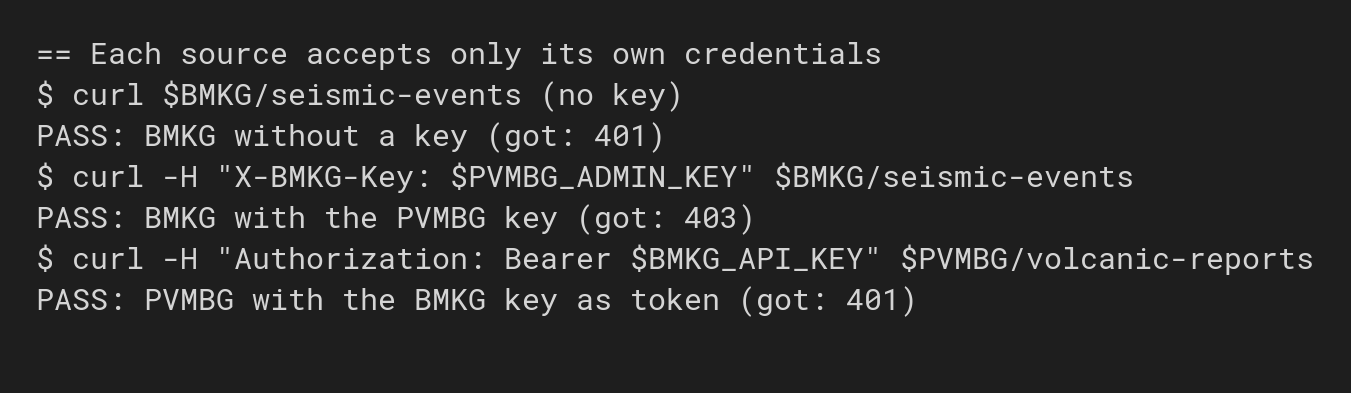
\includegraphics[width=\linewidth,height=0.72\textheight,keepaspectratio]{figures/bukti/viii1.png}
\caption{Kredensial satu instansi dipakai pada instansi lain}
\end{figure}

\subsection{Scope Media Ditolak Akses Field Mentah}

Akun Media hanya menerima field Ringkasan. Permintaan eksplisit terhadap field Mentah ditolak, sedangkan Operator menerima seluruh field.

\begin{figure}[H]
\centering
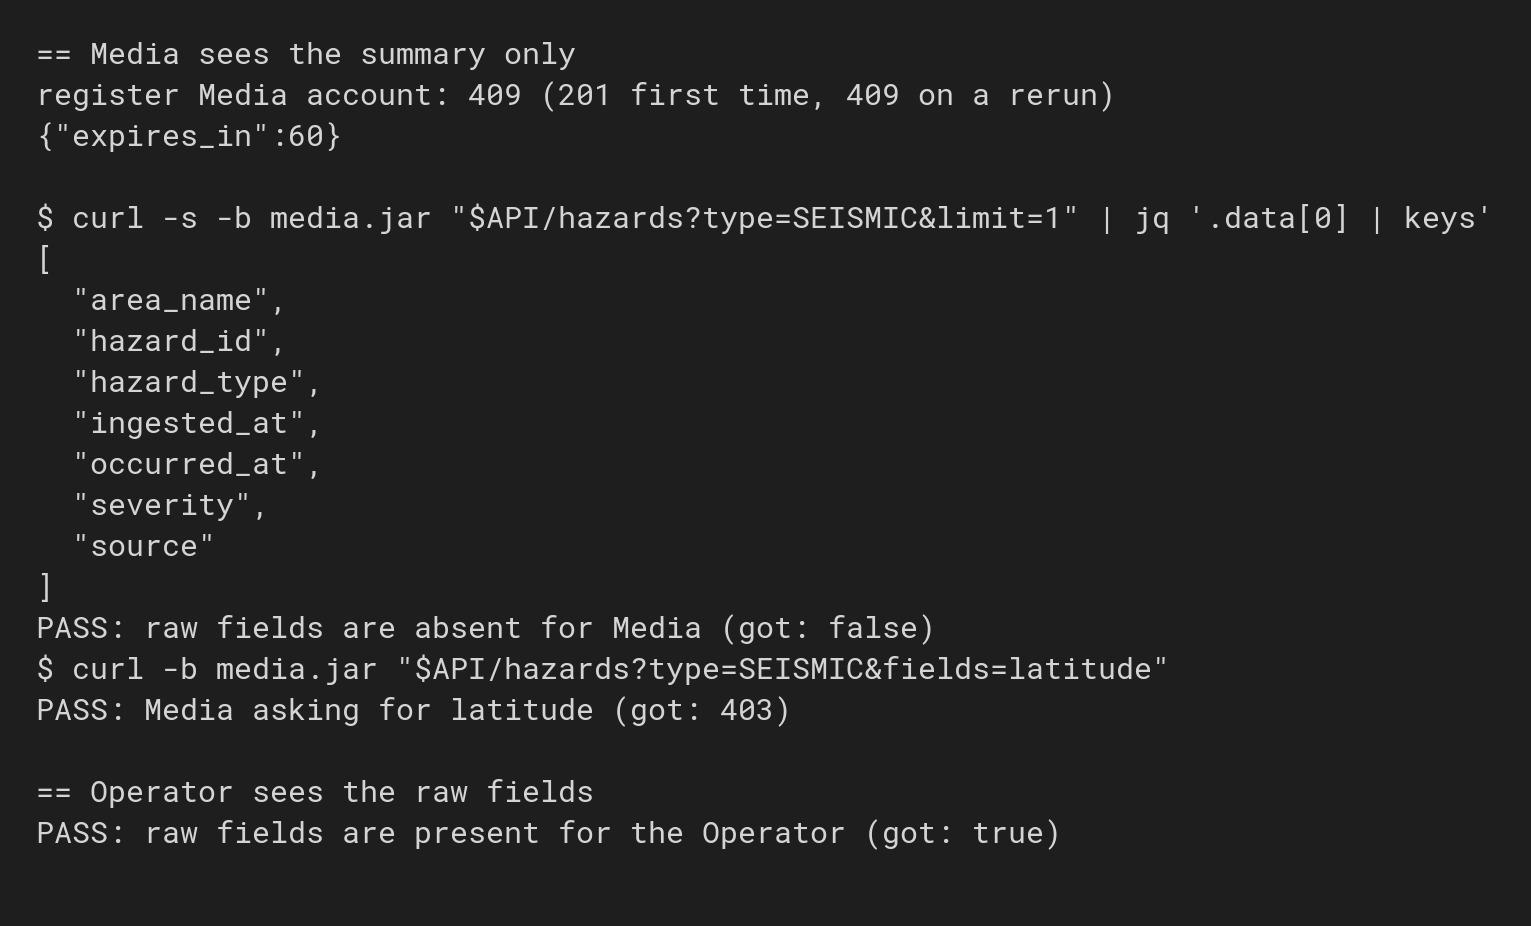
\includegraphics[width=\linewidth,height=0.72\textheight,keepaspectratio]{figures/bukti/viii2.png}
\caption{Field yang terlihat oleh Media dan Operator}
\end{figure}

\subsection{Token Expiry + Refresh Flow Tim Lapangan}

Akun Tim Lapangan login, skrip menunggu 65 detik sampai access token kedaluwarsa, lalu mengirim permintaan berikutnya. Respons 200 membawa cookie \texttt{jwt} dan \texttt{refresh\_token} baru, dan cookie lama ditolak setelah rotasi.

\begin{figure}[H]
\centering
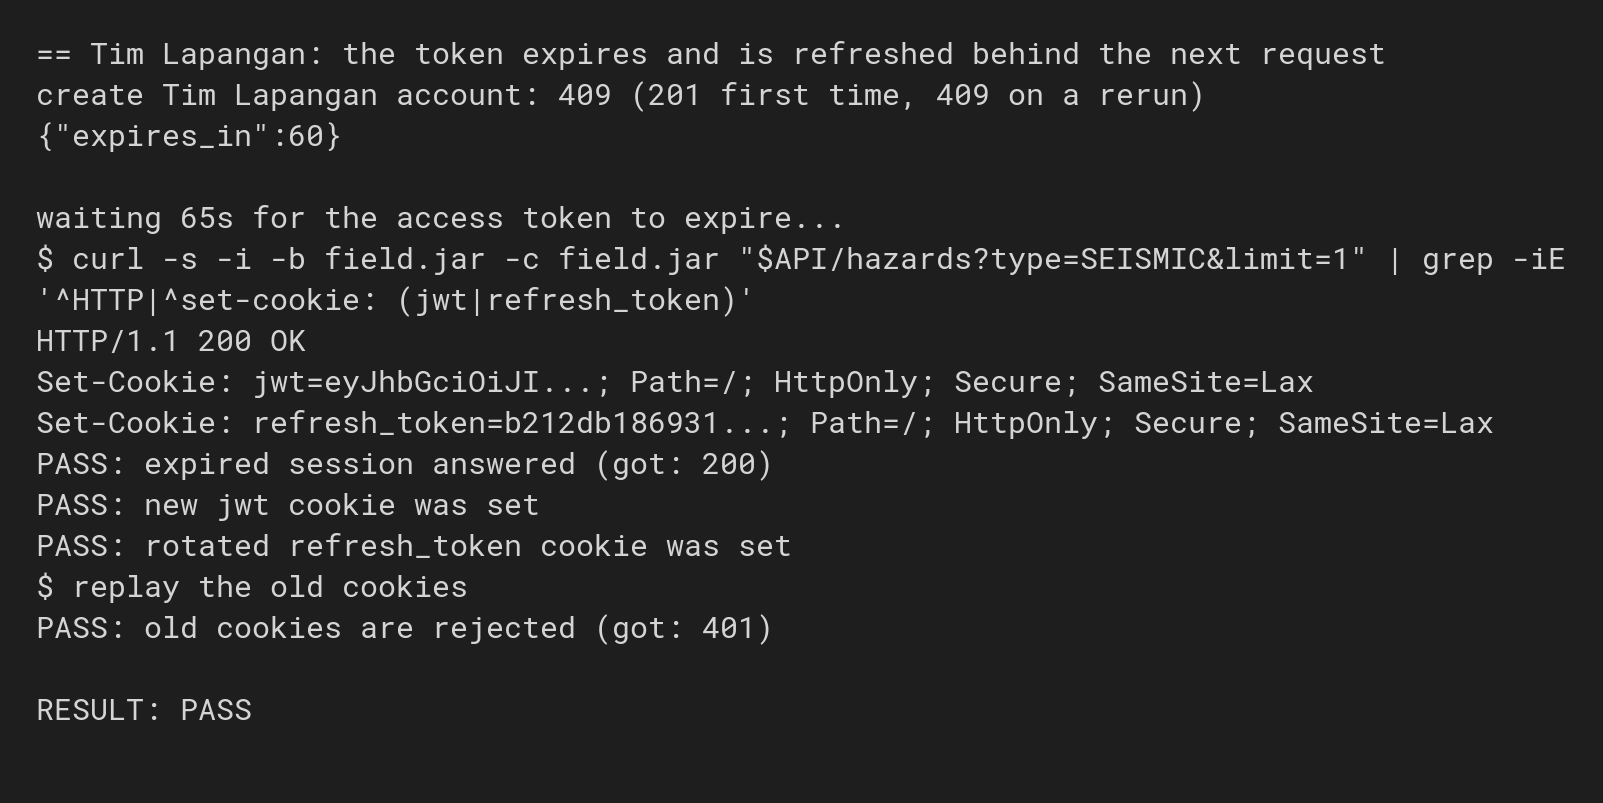
\includegraphics[width=\linewidth,height=0.72\textheight,keepaspectratio]{figures/bukti/viii3.png}
\caption{Kedaluwarsa token dan refresh Tim Lapangan}
\end{figure}

\subsection{Tidak Ada Hardcoded Credential}

Berkas \texttt{.env} berisi nilai asli tidak ikut ter-commit, sedangkan \texttt{.env.example} tersedia. Kode membaca rahasia dari \textit{environment variable}.

\begin{figure}[H]
\centering
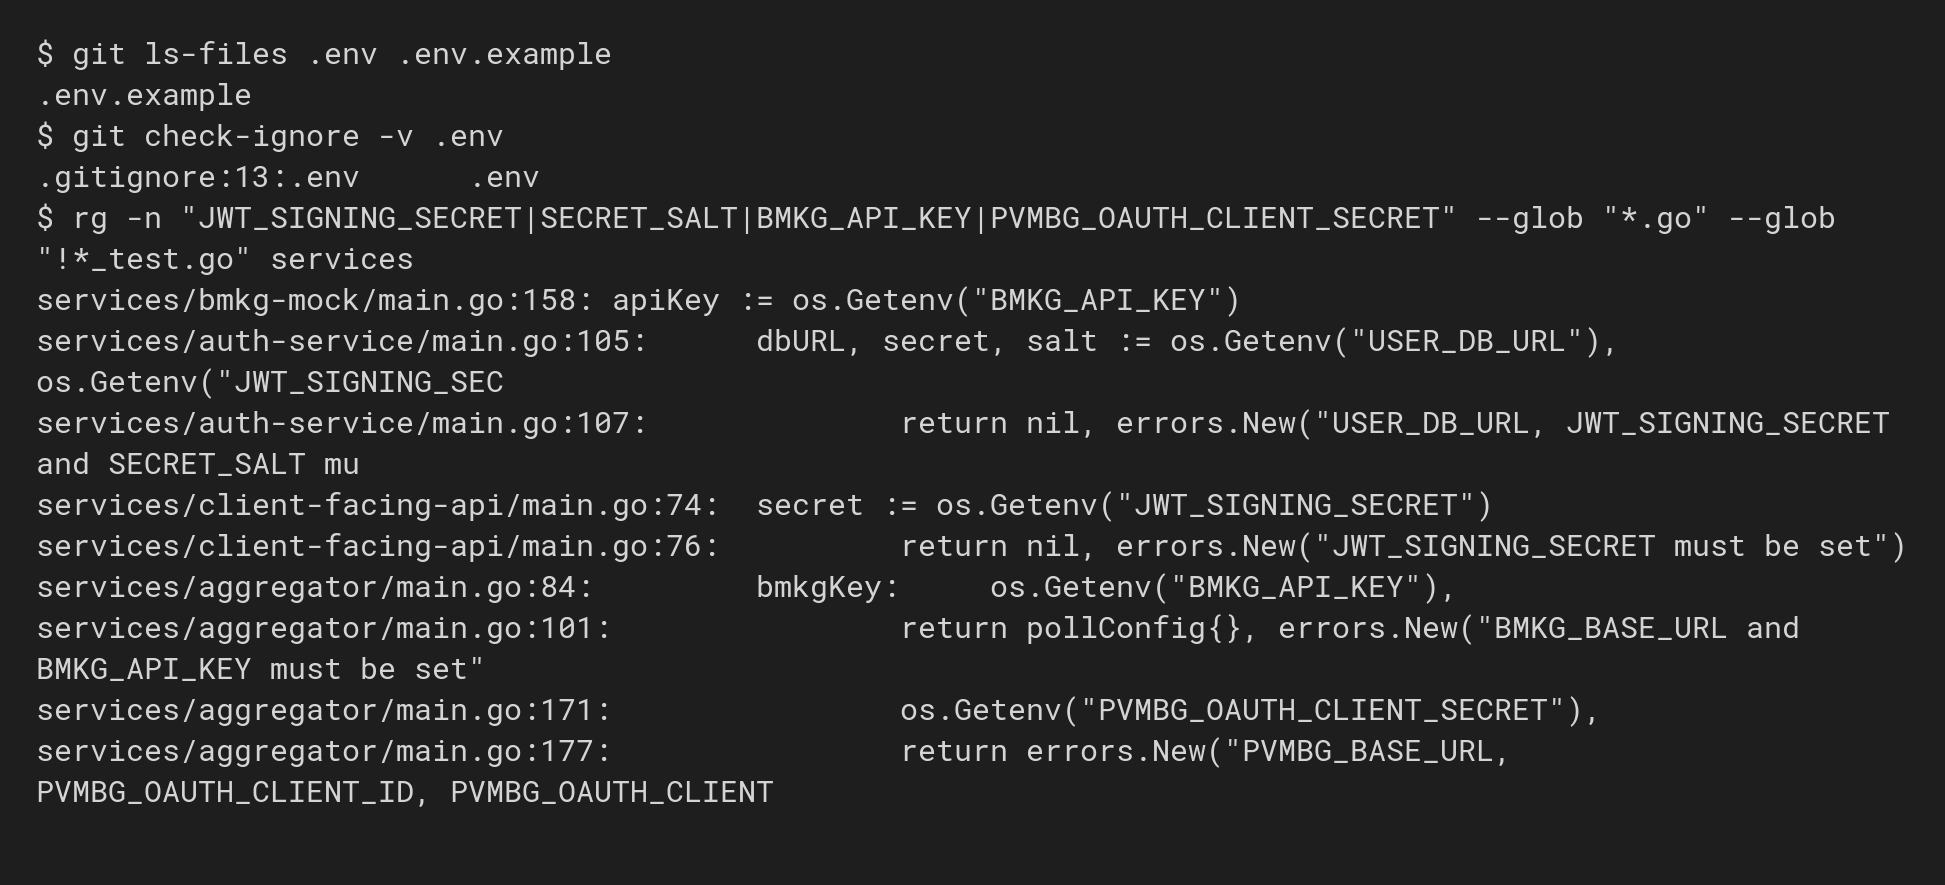
\includegraphics[width=\linewidth,height=0.72\textheight,keepaspectratio]{figures/bukti/viii4.png}
\caption{Pemeriksaan kredensial pada repositori}
\end{figure}

\section{Mekanisme yang Dipakai dan Alasan Tidak Membuka Celah Baru}

Mekanisme terbagi dua. Antara BNPB dan instansi sumber, BNPB mengikuti mekanisme masing-masing: \textit{API key} statis pada header \texttt{X-BMKG-Key} untuk BMKG, dan OAuth 2.0 dengan rotasi \textit{refresh token} untuk PVMBG. Antara \textit{client} dan BNPB, BNPB memakai IdP sendiri yang menerbitkan JWT HS256 dan \textit{refresh token} stateful, keduanya sebagai cookie \textit{HttpOnly}.

Alasan mekanisme ini tidak membuka celah baru adalah sebagai berikut.

\begin{itemize}
\item
  Kredensial tidak dapat dipakai lintas domain. Kunci BMKG ditolak oleh PVMBG dan token PVMBG ditolak oleh BMKG, dengan 401 atau 403. Tidak ada satu kunci pun yang dipakai untuk dua instansi maupun untuk \textit{client} di luar BNPB, sehingga kebocoran satu kredensial tidak membuka sumber lain.
\item
  Tiga \textit{client} adalah tiga identitas dan tiga akun berbeda dengan role tersimpan di User DB, bukan satu akun dengan \textit{flag}. Hak akses ditegakkan di Client-Facing API dari klaim JWT yang sudah diverifikasi: Media hanya menerima field Ringkasan, dan permintaan eksplisit terhadap field Mentah lewat parameter \texttt{fields} dijawab 403 tanpa memanggil Aggregator.
\item
  Token berumur pendek (60 detik secara default) dan \textit{refresh token} dirotasi pada setiap pemakaian, sehingga \textit{refresh token} lama ditolak setelah rotasi. Token curian hanya berguna sampai dipakai atau kedaluwarsa.
\item
  Cookie bertanda \textit{HttpOnly}, \textit{Secure}, dan \textit{SameSite}, sehingga tidak dapat dibaca JavaScript. Setiap 401 pada permintaan bercookie menghapus kedua cookie, karena browser tidak dapat menghapus cookie \textit{HttpOnly} sendiri.
\item
  Kegagalan login dijawab 401 tanpa menyebut email atau kata sandi mana yang salah. Login dan registrasi dibatasi per IP.
\item
  Rahasia tidak ada di kode. Kunci penandatangan JWT, \textit{salt}, kredensial OAuth, dan kunci API dibaca dari \textit{environment variable}, dan repositori hanya memuat \texttt{.env.example} berisi nilai contoh \texttt{change-me*}.
\item
  Aggregator tidak pernah menerbitkan atau menerima token \textit{client}, dan Canonical Store tidak dapat dijangkau dari jaringan mana pun selain milik Aggregator.
\end{itemize}

Batas dari pendekatan ini dicatat pada Batasan yang Disadari, terutama kepercayaan di tepi sistem dan kata sandi yang tidak diperkeras terhadap tebakan luring.

\chapter{Problem 4 - Arsitektur Microservice \& Flexible Storage}

\section{Rancangan Solusi}

Terdapat tiga layanan utama yang relevan dengan Problem 4, yaitu Aggregator, Client-Facing API, dan Auth/Token Service, serta sekelompok event consumer yang terhubung melalui message broker.

Pertama, Aggregator merupakan satu-satunya komponen yang berkomunikasi langsung dengan BMKG dan PVMBG. Komponen ini melakukan polling ke kedua sumber, menerapkan pemetaan yang toleran terhadap perubahan skema sebagaimana didefinisikan pada Problem 1 (field yang tidak dikenal atau baru ditambahkan, seperti confidence\_level, diarahkan ke field attributes), dan merupakan pemilik tunggal Canonical Store. Tidak ada service lain yang memiliki kredensial database maupun connection string ke penyimpanan ini. Selain itu, Canonical Store ditempatkan pada jaringan Docker internal yang hanya diikuti oleh Aggregator, sehingga service lain tidak dapat menjangkaunya secara jaringan.

Kedua, Client-Facing API merupakan proxy read-only. Komponen ini tidak pernah meng-query Canonical Store secara langsung, setiap permintaan data dilayani dengan memanggil API milik Aggregator. Permintaan client diautentikasi dengan memverifikasi JWT secara lokal menggunakan signature dan klaim exp milik token tersebut. Untuk permintaan dengan token yang masih valid, tidak ada panggilan ke Auth/Token Service pada jalur permintaan. Client-Facing API hanya menghubungi Auth/Token Service pada dua kondisi: meneruskan permintaan login, dan melakukan refresh secara transparan ketika access token client telah kedaluwarsa (lihat Bab VIII).

Ketiga, Auth/Token Service bertanggung jawab menerbitkan JWT bertanda tangan dengan TTL pendek yang dapat dikonfigurasi (default 60 detik), serta mengelola refresh token. Komponen ini memiliki penyimpanannya sendiri, yaitu User DB, yang berisi data akun dan refresh token dan tidak diakses oleh service lain. Auth/Token Service tidak memiliki ketergantungan terhadap Aggregator, karena Aggregator tidak pernah menerbitkan maupun mengonsumsi token client. Hubungannya dengan Client-Facing API bersifat satu arah dan terbatas pada login dan refresh.

Terakhir, event consumer (Dashboard, Notifier, dan Audit Logger) berjalan sebagai service terpisah yang berlangganan HazardEvent melalui RabbitMQ. Aggregator hanya mengenal exchange, bukan consumer, sehingga consumer dapat dihentikan, di-rebuild, atau ditambahkan tanpa memengaruhi Aggregator (lihat Problem 5).

HazardEvent disimpan di PostgreSQL dengan skema \emph{hybrid}. Sepuluh field kanonik yang strukturnya ditetapkan spesifikasi (hazard\_id, source, source\_ref\_id, hazard\_type, severity, area\_name, latitude, longitude, occurred\_at, ingested\_at) disimpan sebagai kolom bertipe. Constraint NOT NULL hanya diterapkan pada field wajib (hazard\_id, source, source\_ref\_id, hazard\_type, occurred\_at, ingested\_at), sedangkan field lain bersifat nullable sesuai kebijakan pada Problem 1. Kombinasi (source, source\_ref\_id) diberi unique constraint untuk mencegah duplikasi record akibat polling berulang. Field attributes, yang diperuntukkan bagi atribut spesifik sumber tanpa padanan kanonik, disimpan sebagai kolom JSONB, sehingga field baru seperti confidence\_level dapat tersimpan tanpa migrasi skema.

\section{Alasan Keputusan}

Keputusan pada Problem 4 mencakup dua hal: penentuan batas service dan cara HazardEvent disimpan. Perbandingan alternatif secara lengkap dijabarkan pada Subbab \ref{sec:p4-alternatif}.

\subsection{Batas Service}

Sistem dipecah berdasarkan tanggung jawab fungsional, bukan dipertahankan sebagai monolith. Pada monolith, polling, pemetaan, autentikasi, dan penyajian berada dalam satu unit deploy, sehingga perubahan kecil pada autentikasi memaksa seluruh sistem di-deploy ulang, termasuk bagian pemetaan yang tidak berubah. Pemecahan dilakukan mengikuti tiga pertimbangan:

\begin{itemize}
\tightlist
\item
  Laju perubahan yang berbeda: logika pemetaan berubah mengikuti skema sumber, sedangkan logika autentikasi berubah mengikuti kebijakan keamanan. Keduanya perlu dapat di-deploy terpisah.\\
\item
  Domain of trust yang berbeda: hanya Aggregator yang memegang kredensial BMKG dan PVMBG, dan hanya Auth/Token Service yang memegang kunci penandatanganan token. Pemisahan service membatasi dampak apabila salah satu komponen terkompromi.\\
\item
  Isolasi kegagalan: matinya satu service tidak menghentikan service lain yang tidak bergantung padanya.
\end{itemize}

Salah satu konsekuensi penting dari batas ini adalah verifikasi JWT dilakukan secara lokal di Client-Facing API. Alternatifnya, memanggil Auth/Token Service secara sinkron pada setiap permintaan, ditolak karena menciptakan coupling langsung, restart Auth/Token Service akan melumpuhkan seluruh lalu lintas Client-Facing API. Dengan verifikasi lokal, ketergantungan Client-Facing API terhadap Auth/Token Service terbatas pada login dan refresh. Selama Auth/Token Service di-restart, permintaan dengan token yang masih valid tetap dilayani, hanya login dan refresh yang gagal sementara dan dijawab dengan 503 eksplisit.

\subsection{Independensi Container}

Setiap \textit{service} memiliki Dockerfile sendiri dan didefinisikan sebagai \textit{service} tersendiri di \texttt{docker-compose.yml}. Fondasi independensinya adalah sebagai berikut.

\begin{itemize}
\tightlist
\item
  Jaringan \texttt{canonical-net} dan \texttt{userdb-net} bertanda \texttt{internal}. Masing-masing hanya diikuti oleh pemilik penyimpanannya (Aggregator dan Auth/Token Service) dan penyimpanan itu sendiri.\\
\item
  Setiap penyimpanan punya \textit{volume} sendiri (\texttt{canonical\_store\_data}, \texttt{user\_db\_data}, \texttt{rabbitmq\_data}), begitu pula token OAuth PVMBG dan catatan deduplikasi, sehingga \textit{container} dapat dibuat ulang tanpa kehilangan data.\\
\item
  Setiap \textit{service} punya \textit{healthcheck} dan \texttt{depends\_on} dengan kondisi \texttt{service\_healthy} hanya pada dependensi yang benar-benar dibutuhkan untuk start. Ketiga \textit{consumer} hanya bergantung pada RabbitMQ.\\
\item
  Satu \textit{service} dapat dihentikan, di-\textit{build} ulang, dan dijalankan lagi dengan \texttt{docker compose up -d --build --no-deps --wait <service>}. Opsi \texttt{--no-deps} mencegah dependensinya ikut dibuat ulang.
\end{itemize}

\section{Batasan Yang Disadari}

\subsection{Restart Auth/Token Service berdampak pada login dan refresh}

Permintaan dengan token yang masih valid tetap dilayani, tetapi login dan refresh gagal sementara dengan 503 selama Auth/Token Service di-restart.

\subsection{Aggregator merupakan dependensi utama jalur data}

Restart Aggregator menghentikan sementara ingest dan permintaan data, yang dijawab Client-Facing API dengan 503 eksplisit. Login, refresh, dan consumer tetap berjalan.

\subsection{Canonical Store berjalan sebagai satu instance}

PostgreSQL berjalan tanpa replikasi, sehingga kegagalan database menghentikan jalur data. Data tetap aman karena tersimpan pada Docker volume.

\subsection{Fleksibilitas skema hanya berlaku untuk atribut sumber}

Field baru dari sumber diserap attributes tanpa migrasi, tetapi perubahan format kanonik itu sendiri tetap membutuhkan migrasi. Hal ini dapat diterima karena format kanonik dikendalikan BNPB, bukan instansi sumber.

\subsection{Isi attributes tidak divalidasi dan tidak di-index}\label{sec:p4-attributes}

Kolom attributes menerima tipe nilai apa pun dan belum diberi GIN index. Index dapat ditambahkan kemudian tanpa migrasi data.

\section{Bukti Penyelesaian}

\subsection{Restart Independen Container}

Skenario \texttt{tests/scenarios/problem4.sh} menghentikan Notifier, memastikan service lain tetap berjalan dan API tetap melayani, lalu membangun ulang hanya Notifier. Waktu mulai kontainer Aggregator dan Client-Facing API tidak berubah.

\begin{codebox}
$ docker compose stop notifier
$ docker compose ps --format '{{.Service}} {{.Status}}'
aggregator Up 7 minutes (healthy)      client-facing-api Up 4 minutes (healthy)
audit-logger Up 7 minutes              dashboard-updater Up 7 minutes
(notifier tidak muncul)                rabbitmq Up 7 minutes (healthy)
$ curl -s -b op.jar "$API/hazards?type=SEISMIC&limit=1" | jq '.meta.source_status'
"UP"
$ docker compose up -d --build --no-deps --wait notifier
PASS: notifier is running again
PASS: Aggregator was not restarted (got: 2026-10-09T02:37:03.776899689Z)
PASS: Client-Facing API was not restarted (got: 2026-10-09T02:39:35.822467246Z)
\end{codebox}

\subsection{Record Sebelum/Sesudah Schema Change}

Rekaman PVMBG sebelum dan sesudah perubahan skema tersimpan berdampingan di tabel \texttt{hazard\_events} yang sama tanpa migrasi, seperti pada hasil kueri di Bab VI (\texttt{has\_confidence} bernilai \texttt{f} untuk rekaman lama dan \texttt{t} untuk rekaman baru).

\subsection{Canonical Store Hanya Diakses Aggregator}

Pemeriksaan keterjangkauan dari tiap kontainer ke kedua basis data menunjukkan hanya Aggregator yang menjangkau Canonical Store dan hanya Auth/Token Service yang menjangkau User DB.

\begin{codebox}
aggregator         canonical-store: reachable    user-db: unreachable
auth-service       canonical-store: unreachable  user-db: reachable
bmkg-mock          canonical-store: unreachable  user-db: unreachable
pvmbg-mock         canonical-store: unreachable  user-db: unreachable
rabbitmq           canonical-store: unreachable  user-db: unreachable
client-facing-api  canonical-store: unreachable  user-db: unreachable
web-frontend, dashboard-updater, notifier, audit-logger: kedua basis data unreachable
PASS: only the Aggregator reaches the Canonical Store (got: 1)
PASS: only the Auth Service reaches the User DB (got: 1)
\end{codebox}

\section{Batas Service dan Alternatif Penyimpanan}\label{sec:p4-alternatif}

\subsection{Alternatif Batasan Service}

\begin{longtable}[]{|>{\raggedright\arraybackslash}p{\dimexpr(\linewidth-6\tabcolsep)/3\relax}|>{\raggedright\arraybackslash}p{\dimexpr(\linewidth-6\tabcolsep)/3\relax}|>{\raggedright\arraybackslash}p{\dimexpr(\linewidth-6\tabcolsep)/3\relax}|}
\hline
Pendekatan & Deskripsi & Hasil \\
\hline
\endhead
\endlastfoot
Role Based & Satu service per tanggung jawab fungsional: Aggregator, Client-Facing API, Auth/Token Service, serta consumer terpisah untuk setiap pihak yang berlangganan event. & Dipilih \\
\hline
Monolith & Polling, pemetaan, autentikasi, dan penyajian dalam satu unit deploy. & Ditolak \\
\hline
Source-adapter & Adapter BMKG dan adapter PVMBG terpisah, diikuti service mapper inti. & Ditolak \\
\hline
Pemisahan ingest dan read & Aggregator dipecah menjadi service ingest (polling dan pemetaan) dan service read (melayani query). & Ditolak \\
\hline
Event sourcing / CQRS & HazardEvent disimpan sebagai log append-only, dengan service read-side yang membentuk proyeksi. & Ditolak \\
\hline
\end{longtable}

Monolith (B) ditolak karena perubahan pada satu bagian, misalnya autentikasi, memaksa seluruh sistem di-deploy ulang, termasuk bagian yang tidak berubah. Ini persis masalah yang diangkat Problem 4.

Adapter per sumber (C) memberikan isolasi kegagalan antar-sumber, tetapi isolasi tersebut sudah diperoleh di dalam Aggregator melalui poller independen dan circuit breaker per sumber (Problem 2). Pendekatan ini hanya menambah network hop dan jumlah service tanpa manfaat tambahan pada cakupan dua sumber.

Pemisahan ingest dan read (D) ditolak karena kedua service akan membutuhkan akses langsung ke Canonical Store, sehingga melanggar ketentuan bahwa setiap storage dimiliki tepat satu service. Alasan inilah yang membuat ingest dan penyajian data tetap berada dalam satu batas service, yaitu Aggregator.

Event sourcing / CQRS (E) ditolak karena menambah kompleksitas pemeliharaan log dan proyeksi, serta memperkenalkan jeda konsistensi antara keduanya, tanpa kebutuhannya untuk sekarang. Kebutuhan distribusi event sudah dipenuhi oleh message broker pada Problem 5.

\subsection{Alternatif Penyimpanan Canonical Store}

\begin{longtable}[]{|>{\raggedright\arraybackslash}p{\dimexpr(\linewidth-10\tabcolsep)/5\relax}|>{\raggedright\arraybackslash}p{\dimexpr(\linewidth-10\tabcolsep)/5\relax}|>{\raggedright\arraybackslash}p{\dimexpr(\linewidth-10\tabcolsep)/5\relax}|>{\raggedright\arraybackslash}p{\dimexpr(\linewidth-10\tabcolsep)/5\relax}|>{\raggedright\arraybackslash}p{\dimexpr(\linewidth-10\tabcolsep)/5\relax}|}
\hline
Aspek & PostgreSQL + JSONB (dipilih) & Relasional kolom tetap & Document store (MongoDB) & Key-value store (Redis) \\
\hline
\endhead
\endlastfoot
Field baru (confidence\_level) & Diserap kolom JSONB attributes, tanpa migrasi & Wajib migrasi (ALTER TABLE) dan deploy bersama & Diserap secara native, tanpa migrasi & Diserap secara native, tanpa migrasi \\
\hline
Validasi field kanonik (severity, hazard\_type) & Bawaan definisi tabel melalui ENUM, CHECK, dan NOT NULL & Bawaan definisi tabel & Tersedia melalui json schema, tetapi opsional dan dikonfigurasi terpisah & Tidak tersedia, sepenuhnya di level aplikasi \\
\hline
Deduplikasi (source, source\_ref\_id) & UNIQUE constraint bawaan & UNIQUE constraint bawaan & Unique index & Hanya melalui desain key, tanpa jaminan atomik lintas operasi \\
\hline
Query field kanonik (hazard\_type, severity, occurred\_at) & B-tree index bawaan & B-tree index bawaan & Secondary index didukung & Tidak didukung secara native, index harus dibangun dan dirawat manual \\
\hline
Query berdasarkan isi attributes & Dapat ditambahkan melalui GIN index tanpa migrasi data & Tidak berlaku (tidak ada kolom fleksibel) & Didukung secara native & Tidak didukung, harus membaca setiap value \\
\hline
\end{longtable}

PostgreSQL dengan JSONB dipilih karena merupakan satu-satunya opsi yang sekaligus menyerap field baru tanpa migrasi dan menegakkan validasi serta deduplikasi field kanonik sebagai bagian bawaan dari definisi tabel. Relasional dengan kolom tetap memberikan validasi yang sama, tetapi setiap field baru dari sumber mewajibkan migrasi, sehingga coupling dari Problem 1 muncul kembali melalui jalur storage. Document store memenuhi kebutuhan tanpa migrasi dan dapat melakukan validasi melalui \emph{jsonSchema}, tetapi validasi tersebut bersifat opsional dan terpisah dari penyimpanan data, sedangkan fleksibilitas skema penuhnya tidak dibutuhkan karena hanya attributes yang berubah-ubah. Key-value store paling sederhana, tetapi tidak mendukung query berdasarkan field selain key, padahal Client-Facing API membutuhkan filter berdasarkan hazard\_type dan waktu.

Konsekuensi dari pilihan ini adalah dua model data dalam satu tabel, field kanonik tervalidasi ketat, sedangkan isi attributes tidak tervalidasi di tingkat database (lihat Subbab \ref{sec:p4-attributes}).

\chapter{Problem 5 - Fan-out Event Distribution/Pub-sub}

\section{Rancangan Solusi}

Aggregator mempublikasikan HazardEvent ke RabbitMQ melalui satu fanout exchange. Hanya HazardEvent yang baru atau berubah berdasarkan hasil upsert ke Canonical Store yang dipublikasikan, sehingga data yang diterima ulang akibat polling berulang tidak dipublikasikan kembali. Correlation ID dibawa melalui properti AMQP correlation\_id, terpisah dari payload HazardEvent.

Setiap consumer (Dashboard Updater, Notifier, dan Audit Logger) mendeklarasikan durable queue miliknya sendiri dan mengikatnya ke exchange tersebut. Tidak ada queue yang dibagi antar-consumer, sehingga setiap consumer menerima salinan dari setiap pesan. Aggregator hanya mengenal nama exchange dan tidak mengetahui keberadaan consumer. Audit Logger digunakan untuk mendemonstrasikan penambahan consumer baru tanpa perubahan kode producer.

Di sisi producer, publish() memasukkan pesan ke buffer in-memory berukuran terbatas dan langsung mengembalikan kendali, sehingga loop polling Aggregator tidak menunggu broker. Task latar belakang mengirim pesan dengan publisher confirms dan melakukan retry saat gagal. Jika buffer penuh akibat outage broker yang berkepanjangan, pesan tertua dibuang dan dicatat ke log beserta hazard\_id-nya.

Queue dideklarasikan sebagai durable dan pesan dipublikasikan sebagai persistent (delivery\_mode = 2), sehingga pesan yang terbit saat consumer mati tetap tersimpan di queue dan diproses setelah consumer menyala kembali.

Seluruh consumer menggunakan manual acknowledgment: pesan baru di-ack setelah selesai diproses, sehingga pesan yang sedang diproses saat consumer crash akan dikirim ulang. Karena redelivery dapat menghasilkan duplikat, setiap consumer dibuat idempoten: - Dashboard Updater melakukan upsert ke state map in-memory berkunci hazard\_id, sehingga memproses pesan yang sama dua kali menghasilkan state yang sama. - Notifier dan Audit Logger mencatat pasangan (hazard\_id, severity) yang sudah diproses, dan melewati pesan dengan pasangan yang sudah tercatat. Penggunaan severity dalam kunci memastikan eskalasi tingkat ancaman pada event yang sama, misalnya dari SIAGA menjadi AWAS, tetap diproses.

Catatan (hazard\_id, severity) disimpan pada berkas di disk milik masing-masing consumer. Agar pemeriksaan tidak dibebani latensi I/O, isi berkas dimuat ke memori setiap kali service dinyalakan, dan pemeriksaan dilakukan terhadap data di memori. Setelah pesan berhasil diproses, catatan ditambahkan ke memori sekaligus ditulis ke disk, baru kemudian pesan di-ack. Dengan demikian, catatan tetap ada setelah crash dan restart.

\section{Alasan Keputusan}

\subsection{Pemilihan Broker}

RabbitMQ, Kafka, and NATS were each evaluated against the five Problem 5 criteria and against the team's operational constraints under a fixed deadline.

\begin{longtable}[]{|>{\raggedright\arraybackslash}p{\dimexpr(\linewidth-8\tabcolsep)/4\relax}|>{\raggedright\arraybackslash}p{\dimexpr(\linewidth-8\tabcolsep)/4\relax}|>{\raggedright\arraybackslash}p{\dimexpr(\linewidth-8\tabcolsep)/4\relax}|>{\raggedright\arraybackslash}p{\dimexpr(\linewidth-8\tabcolsep)/4\relax}|}
\hline
Aspek & RabbitMQ (dipilih) & Kafka & NATS (core) \\
\hline
\endhead
\endlastfoot
Fan-out ke consumer independen & Fanout exchange bawaan & Consumer group terpisah per consumer & Subscription terpisah \\
\hline
Catch-up setelah consumer restart & Durable queue dan persistent message & Offset consumer group & Tidak didukung tanpa JetStream \\
\hline
History event untuk consumer baru & Tidak ada & Ada, sesuai log retension & Tidak ada tanpa JetStream \\
\hline
Kebutuhan Spesifikasi (M1) & Satu container, ringan & Lebih berat (KRaft, Partition) & Paling ringan, sampai JetSream diaktifkan \\
\hline
\end{longtable}

RabbitMQ dipilih karena mendukung at-least-once secara bawaan (durable queue, persistent message, publisher confirms) dan fanout exchange-nya sesuai langsung dengan kebutuhan distribusi ke banyak consumer. Keunggulan Kafka dalam menyediakan history event bagi consumer baru tidak dibutuhkan pada M1, karena history HazardEvent sudah tersedia melalui API Aggregator.

\subsection{Jenis Exchange}

Topic exchange dengan pola catch-all, berperilaku sama dengan fanout pada kebutuhan saat ini, tetapi menambah beban merancang skema routing key yang belum terpakai. Fanout dipilih karena lebih sederhana, dan peralihan ke topic exchange tetap dapat dilakukan kemudian.

\subsection{Queue per Consumer}

Consumer yang berbagi satu queue akan menerima pesan secara bergiliran, sehingga setiap pesan hanya sampai ke satu consumer. Queue per consumer memastikan setiap consumer menerima setiap event.

\subsection{Kebijakan Buffer Producer}

Buffer tanpa batas berisiko menghabiskan memori saat outage broker, sedangkan buffer yang memblokir membuat producer tertahan. Buffer terbatas yang membuang pesan tertua dipilih karena event terbaru lebih relevan secara operasional, dan event yang dibuang tetap tersimpan di Canonical Store.

\subsection{Manual Acknowledgement}

Automatic acknowledgment menyebabkan pesan hilang bila consumer crash di tengah pemrosesan. Manual acknowledgment dipilih karena kehilangan HazardEvent lebih berbahaya daripada duplikat, dengan konsekuensi setiap consumer wajib idempoten.

\subsection{Kunci Deduplikasi}

Kunci hazard\_id saja membuat eskalasi severity pada event yang sama, misalnya SIAGA menjadi AWAS, dianggap duplikat dan tidak diproses. Kunci (hazard\_id, severity) menangani kasus ini tanpa menambah field pada format kanonik.

\subsection{Penyimpanan Status Deduplikasi}

Pemeriksaan langsung ke disk menambah latensi I/O, sedangkan penyimpanan hanya di memori hilang saat crash, yang justru memicu redelivery. Karena itu, catatan dimuat dari disk ke memori saat service dinyalakan, diperiksa di memori, dan ditulis ke keduanya sebelum pesan di-ack.

\section{Batasan Yang Disadari}

\begin{enumerate}
\def\labelenumi{\arabic{enumi}.}
\tightlist
\item
  Event dapat tidak terpublikasi saat broker atau Aggregator bermasalah Jika outage broker melebihi kapasitas buffer, pesan tertua dibuang. Buffer juga berada di memori, sehingga pesan yang belum terkirim hilang bila Aggregator crash. Event tersebut tetap tersimpan di Canonical Store, tetapi tidak dipublikasikan ulang karena pola outbox tidak diterapkan.\\
\item
  Consumer baru tidak menerima riwayat event Queue dideklarasikan oleh consumer saat pertama kali dijalankan, sehingga event yang terbit sebelum itu tidak diterima. Riwayat HazardEvent tetap dapat diperoleh melalui API Aggregator.\\
\item
  Queue consumer yang mati dapat tumbuh tanpa batas Selama consumer mati, pesan terus menumpuk di queue-nya karena batas panjang queue maupun TTL pesan tidak dikonfigurasi.\\
\item
  Duplikat masih mungkin terjadi Jika consumer crash setelah memproses pesan tetapi sebelum catatan deduplikasi tersimpan, pesan tersebut akan diproses ulang setelah redelivery, misalnya peringatan terkirim dua kali. Konsekuensi ini diterima karena peringatan ganda lebih aman daripada peringatan yang terlewat.\\
\item
  State Dashboard Updater hilang saat restart State map disimpan di memori dan hanya terbentuk kembali dari event yang diterima setelah restart. Sinkronisasi ulang dari API Aggregator saat start tidak diimplementasikan.\\
\item
  Kunci deduplikasi tidak menangani severity yang naik kembali Dengan kunci (hazard\_id, severity), jika severity sebuah event turun lalu naik kembali ke tingkat yang pernah diproses, misalnya SIAGA menjadi WASPADA lalu kembali SIAGA, kenaikan kedua dianggap duplikat. Pola perubahan ini dinilai jarang terjadi pada cakupan M1.\\
\item
  Catatan deduplikasi tidak pernah dibersihkan Berkas catatan (hazard\_id, severity) terus bertambah dan dimuat seluruhnya ke memori setiap kali service dinyalakan. Pada skala M1 ukurannya tidak signifikan.\\
\item
  RabbitMQ berjalan sebagai satu instance Broker berjalan tanpa clustering, sehingga selama broker mati distribusi event terhenti. Pesan yang sudah berada di queue tetap aman karena bersifat persistent dan tersimpan pada Docker volume.
\end{enumerate}

\section{Bukti Penyelesaian}

\subsection{Publish ke Broker}

\textless placeholder\textgreater{}

\subsection{Dua Consumer Independen}

\textless placeholder\textgreater{}

\subsection{Case Consumer Mati}

\textless placeholder\textgreater{}

\subsection{Penambahan Consumer Baru Tanpa Ubah Producer}

\textless placeholder\textgreater{}

\section{Broker, Pola, dan Semantik Pengiriman}

\subsection{Broker dan Pola}

Sistem menggunakan RabbitMQ dengan pola publish-subscribe berbasis fanout exchange. Setiap consumer memiliki durable queue sendiri yang terikat ke exchange, sehingga setiap consumer menerima setiap HazardEvent secara independen dari consumer lain.

\subsection{Semantik Pengiriman}

Semantik pengiriman dibedakan untuk dua jalur:

\begin{itemize}
\tightlist
\item
  Producer ke broker: at-least-once melalui publisher confirms dan retry. Semantik ini turun menjadi at-most-once hanya bila outage broker berlangsung melebihi kapasitas buffer, karena pesan tertua dibuang dan dicatat ke log.\\
\item
  Broker ke consumer: at-least-once untuk seluruh consumer melalui manual acknowledgment. Pesan yang sedang diproses saat consumer crash akan dikirim ulang, dan pesan yang terbit saat consumer mati tetap tertampung di durable queue hingga consumer menyala kembali.
\end{itemize}

\subsection{Konsekuensi bagi Consumer}

Karena pengiriman bersifat at-least-once, consumer dapat menerima pesan yang sama lebih dari sekali, sehingga setiap consumer wajib idempoten:

\begin{itemize}
\tightlist
\item
  Dashboard Updater: upsert ke state map berkunci hazard\_id, sehingga pesan duplikat menghasilkan state yang sama.\\
\item
  Notifier dan Audit Logger: melewati pesan dengan pasangan (hazard\_id, severity) yang sudah tercatat. Catatan disimpan di disk dan dimuat ke memori saat service dinyalakan, sehingga tetap berlaku setelah crash dan restart.
\end{itemize}

Duplikat masih dapat terjadi bila consumer crash setelah memproses pesan tetapi sebelum catatannya tersimpan. Konsekuensi ini diterima karena peringatan ganda lebih aman daripada peringatan yang terlewat.

\chapter*{Deklarasi Penggunaan LLM}
\addcontentsline{toc}{chapter}{Deklarasi Penggunaan LLM}

\subsection{Subbab}

\textless placeholder\textgreater{}

\subsection{Subbab}

\textless placeholder\textgreater{}

\chapter*{REFERENSI}
\addcontentsline{toc}{chapter}{REFERENSI}

\hangindent=1.27cm \hangafter=1 Broadcom. (n.d.). \textit{RabbitMQ tutorial: Publish/Subscribe}. RabbitMQ. Retrieved October 9, 2026, from \url{https://www.rabbitmq.com/tutorials/tutorial-three-go}

\hangindent=1.27cm \hangafter=1 Cuervo, A. F. (2016). Handling overload. In B. Beyer, C. Jones, J. Petoff, \& N. R. Murphy (Eds.), \textit{Site reliability engineering}. O'Reilly Media. Retrieved October 9, 2026, from \url{https://sre.google/sre-book/handling-overload/}

\hangindent=1.27cm \hangafter=1 Fowler, M. (2014, March 6). \textit{CircuitBreaker}. martinfowler.com. Retrieved October 9, 2026, from \url{https://martinfowler.com/bliki/CircuitBreaker.html}

\hangindent=1.27cm \hangafter=1 Hardt, D. (Ed.). (2012, October). \textit{The OAuth 2.0 authorization framework}~(RFC 6749). Internet Engineering Task Force. Retrieved October 9, 2026, from \url{https://www.rfc-editor.org/rfc/rfc6749}

\hangindent=1.27cm \hangafter=1 Jones, M., Bradley, J., \& Sakimura, N. (2015, May). \textit{JSON Web Token (JWT)}~(RFC 7519). Internet Engineering Task Force. Retrieved October 9, 2026, from \url{https://www.rfc-editor.org/rfc/rfc7519}

\hangindent=1.27cm \hangafter=1 Jones, M., \& Hardt, D. (2012, October). \textit{The OAuth 2.0 authorization framework: Bearer token usage}~(RFC 6750). Internet Engineering Task Force. Retrieved October 9, 2026, from \url{https://www.rfc-editor.org/rfc/rfc6750}

\hangindent=1.27cm \hangafter=1 Paani, R. (2023, December 9). \textit{Using Protocol Buffer's (protobuf) Struct datatype for generic objects/JSON representation}. Medium. Retrieved September 26, 2026, from \url{https://medium.com/@raj.paani/using-protocol-buffers-protobuf-struct-datatype-for-generic-objects-json-representation-57bc1ba5c248}

\hangindent=1.27cm \hangafter=1 PostgreSQL Global Development Group. (n.d.). \textit{JSON types}. PostgreSQL 16 Documentation. Retrieved October 9, 2026, from \url{https://www.postgresql.org/docs/16/datatype-json.html}

\hangindent=1.27cm \hangafter=1 PT Cipta Piranti Sejahtera. (2026, June 11). \textit{Otentikasi dan otorisasi OAuth}. Dokumentasi Integrasi API Accurate Online. Retrieved September 28, 2026, from \url{https://accurate.id/api-integration/oauth/}

\hangindent=1.27cm \hangafter=1 roger. (2015, August 12). \textit{How can I define a map accept different kind of value in thrift?} Stack Overflow. Retrieved September 26, 2026, from \url{https://stackoverflow.com/questions/31958381/how-can-i-define-a-map-accept-different-kind-of-value-in-thrift}

\hangindent=1.27cm \hangafter=1 The VitalVas. (2026, June 23). \textit{JWT vs opaque access tokens}. Blog Notes. Retrieved September 28, 2026, from \url{https://blog.vitalvas.com/post/2026/06/23/jwt-vs-opaque-access-tokens/}

\hangindent=1.27cm \hangafter=1 W3C. (2021, November 23). \textit{Trace context}. W3C Recommendation. Retrieved October 9, 2026, from \url{https://www.w3.org/TR/trace-context/}


\end{document}
